\documentclass[12pt,a4paper]{article}
\usepackage[utf8]{inputenc}
\usepackage{amsmath}
\usepackage{amsfonts}
\usepackage{amssymb}
\usepackage{graphicx}
\usepackage{enumerate}
\usepackage{amsthm}
\usepackage[a4paper, total={6in, 8in}]{geometry}
\usepackage{listings}
\usepackage{tikz}
\usepackage{tikz-cd}
\usepackage{epstopdf}
\usepackage{hyperref}
\usepackage{subcaption}
\usepackage{color}
\usepackage[bottom, hang]{footmisc}

\numberwithin{equation}{section}

\newtheorem{lemma}{Lemma}[section]

\newtheorem{theorem}{Theorem}[section]
\newtheorem{corollary}{Corollary}[section]

\theoremstyle{definition}
\newtheorem{definition}{Definition}[section]

\newtheorem{proposition}{Proposition}[section]

\newtheorem{example}{Example}[section]

\theoremstyle{remark}
\newtheorem{remark}{Remark}

\lstset{basicstyle=\ttfamily,
language=Matlab,showspaces=false,frame=single,breaklines=true,showstringspaces=false,
numbers=left,numberstyle={\tiny \color{black}},numbersep=9pt}

\setcounter{secnumdepth}{5}

\usepackage[numbib,nottoc]{tocbibind}

\begin{document}
%\textbf{\textcolor{red}{TODO:}}
%\begin{itemize}
%\item 23:00 - Generalisations
%\item Wed Night - Hopf maps?
%\end{itemize}
%\pagebreak

\vspace{1cm}
\title{    
    \textsc{Results on the \\Parallelisability of Spheres}
    }
    
    \vspace{1cm}
    
    % if you are the only author, you might use the following
    \author{Rhuaidi Antonio Burke}  
    
    % Insert here your name and correct mail address
    %\author{\Large \href{mailto:first.student@smail.fh-koeln.de}{First Student} \and \Large \href{mailto:second.student@smail.fh-koeln.de}{Second Student}
    \vspace{1cm}
    
    % name of the course and module
    \date{
    \large SCIE3250 \\ Final Report \\ 
    \vspace{1cm}
    \large Supervisor: Dr. Paul Bryan \\
    \vspace{1cm}
    \today
    }

    \maketitle
    \setlength{\parindent}{0pt}

\vspace{2cm}
\begin{abstract}
\noindent This report discusses parallelisability of spheres. The first section gives a review of some of the concepts from differential geometry used. Using techniques from analysis due to Milnor, we then present a proof that $\mathbb{S}^n$ admits no non-vanishing vector field for even $n$. This result is then used to prove the ``Hairy Ball Theorem''. The Poincar\`{e}-Hopf theorem is also proven for general manifolds. From this, we then present a different proof regarding the existence of the aforementioned vector fields.
We then show that $\mathbb{S}^1$, $\mathbb{S}^3$ and $\mathbb{S}^7$ are parallelisable by directly constructing 1, 3 and 7 smooth linearly independent, nowhere vanishing vector fields on each of these spheres respectively. The connection of this result to the existence of normed division algebras is then considered. Consequences and generalisations of these results are also briefly discussed, in particular the existence of Hopf maps and the work of Adams.\\
\begin{center}
\noindent All graphics were made in either Adobe Illustrator or Mathematica unless otherwise stated.
\end{center}
\end{abstract}


%\title{Results on the Parallelisability of Spheres}
%\author{Rhuaidi Burke,\\Under the supervision of Dr. Paul Bryan.}
%\maketitle
%\begin{abstract}
%%An interesting question to ask when working with smooth manifolds is how many smooth pointwise linearly independent vector fields can place on the manifold. If the number of vector fields is equal to the dimension of the manifold, we say the manifold is parallelisable. 
%This report discusses parallelisability of spheres. The first section gives a review of some of the concepts from differential geometry used. Using techniques from analysis due to Milnor, we then prove that $\mathbb{S}^n$ admits no non-vanishing vector field for $n$ even and as a result, prove the well-known ``Hairy Ball Theorem''. We also prove the Poincar\`{e}-Hopf theorem for both regular surfaces and general manifolds. From this, we then present a different proof regarding the existence of the aforementioned vector fields.
%We then show that $\mathbb{S}^1$, $\mathbb{S}^3$ and $\mathbb{S}^7$ are parallelisable by directly constructing 1, 3 and 7 smooth linearly independent vector fields on each of these spheres respectively. The connection of this result to the existence of the Hopf maps and division algebras are then considered. Consequences and generalisations of these results are also discussed.\\
%
%\begin{flushleft}
%All graphics original and painstakingly made in Adobe Illustrator or Mathematica unless otherwise stated.
%\end{flushleft}
%\end{abstract}
\thispagestyle{empty}
\nocite{*}
\pagebreak
\tableofcontents
\pagebreak
%\listoffigures

%\listoftables
%\pagebreak
\section{Introduction}
The primary area of study that this research project takes place in is differential geometry and topology. One of the most important concepts, not just in differential geometry and topology, but in almost all areas of mathematics, is that of a \textit{manifold}. At this point, it will suffice if the reader considers the surface of a sphere or torus.\\

\begin{figure}[h!]
\centering
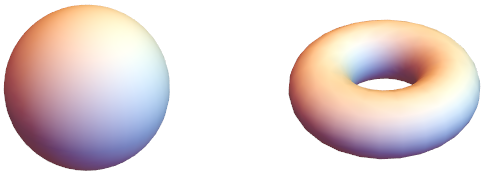
\includegraphics[scale=0.675]{fig/fig1a}
\caption{The sphere and torus are examples of manifolds.}
\end{figure}

If one were to cut out a small piece of one of these surfaces, then it would look like a flat sheet of paper. Since this sheet of paper is two-dimensional, we think of these surfaces as being two-dimensional as well. What makes the study of manifolds interesting however, is in what is happening at a \textit{global} scale: \textit{locally} a piece of the sphere looks like the flat Euclidean plane but \textit{globally} the sphere is clearly not flat and standard notions from Euclidean geometry no longer apply. For example, if one takes two parallel lines on the surface of a sphere (where a ``line'' is no longer necessarily a straight line but still has the meaning of shortest path between two points) and continue along them for long enough, they will eventually meet. For instance, imagine two lines that point due north from the equator - they will start out parallel but will intersect at the north pole.\\

\begin{figure}[h!]
\centering
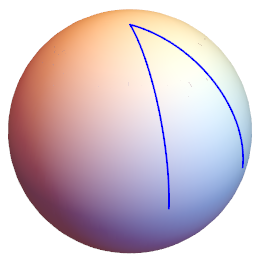
\includegraphics[scale=0.675]{fig/fig2a}
\caption{Two lines starting out parallel on the sphere will eventually intersect.}
\end{figure}

These examples of the sphere and torus are usually visualised quite naturally as surfaces ``sitting'' in three-dimensional space but often we will talk about manifolds as intrinsic objects - not necessarily embedded in any higher space. Furthermore, there is nothing stopping us from talking about manifolds of any arbitrary dimension, and while a seven dimensional sphere may be hard to visualise, such higher-dimensional objects are of central importance to this project.\\

\pagebreak

One important task when working with abstract manifolds is the choice of a local coordinate system so that explicit computations may be carried out on the manifold. As a motivating example, consider $\mathbb{S}^2$. We can think of each point on $\mathbb{S}^2$ as the origin of its tangent space. One must decide how to draw an $x$-axis and a $y$-axis, as well as the positive and negative directions along each axis. This information can be encoded by two arrows, one pointing along the $x$-axis in the positive direction and one pointing along the $y$-axis in the positive direction. A natural question to ask arises, namely:
\begin{center}
\textit{Can we choose our arrows at each point of our space in such a way that they vary smoothly when the points themselves vary smoothly?}
\end{center} 
If we can make such a choice, our space is said to be \textit{parallelisable}.

In Section 3.1, in the case of $\mathbb{S}^2$, it is show that such a choice cannot be made. It is then shown that this is in fact true of all even dimensional spheres. Furthermore, we will find that the only spheres that do admit such a choice are $\mathbb{S}^1$, $\mathbb{S}^3$ and $\mathbb{S}^7$. Strictly speaking $\mathbb{S}^0$ also admits such a choice, however is considered a trivial case.

%Fundamentally, we are interested in answering the question:
%\begin{center}
%\textit{Which spheres admit a parallelisation?}
%\end{center}
\subsection{Literature Review and Historical Overview}
As previously stated, a classic result of algebraic topology due to Brouwer in 1912 \cite{MR1511678} is that in the case of the two-dimensional sphere $\mathbb{S}^2$, we cannot make such a choice. This result came to be known as the ``Hairy Ball Theorem'', since it can be thought of as saying that there is no way to comb the hair of a coconut (or someone's head) without creating a cowlick. It is also worth noting that Brouwer's original proof made use of cohomology theory and other tools from algebraic topology \cite{MR1415833}. Milnor gave a new, more analytic, proof of the theorem in 1978 \cite{MR505523}.\\

One of the results that we will show in the latter sections of this report is that this result generalises, in that it is not possible to make such a choice of arrows on any sphere of even dimension (equivalently, only spheres of odd dimension admit the existence of, at least one, everywhere non-zero smooth vector field). 
%The proof presented is due mainly to \cite{burger2016riemannian} and is nice in its use of relatively elementary differential geometry and analytic methods.\\
What we find in the case of $\mathbb{S}^3$ the three-dimensional sphere however, is quite different. We can think of $\mathbb{S}^3$ as the collection of all points of the form $(x,y,z,w)$ unit distance from the origin, such that $x^2+y^2+z^2+w^2=1$. Each point of the 3-sphere can now be regarded as an object known as a \textit{quaternion}, which are a type of number developed in 1843 by William Hamilton \cite{hamilton1844ii}.\\

Quaternions are similar in nature to complex numbers, but we now introduce three distinct numbers, denoted usually by $i,j,k$, each with the property $i=j=k=\sqrt{-1}$. Unlike real or complex numbers however, the order in which one multiplies quaternions matters; this is to say that $ij=k$ but $ji=-k$. The quaternion associated with the point $(x,y,z,w)$ is $x+yi+zj+wk$ and if $x^2+y^2+z^2+w^2=1$, then it is called a \textit{union quaternion}.
It can be shown that multiplying two unit quaternions together results in another unit quaternion. Furthermore, given any unit quaternion $q$, the three (unit) quaternions given by $iq$, $jq$ and $kq$ are all perpendicular to $q$. Therefore, one can use these quaternions as directions for the three axes needed for the tangent space at $q$ and that they do vary smoothly as the point $q$ varies.\\

One may then be curious as to whether this type of construction generalises to higher dimension. That is, through some notion of `nice multiplication' of points on the sphere. Assuming we wish to use a conventional number system, we have at our disposal the real numbers, the complex numbers (which give us a result for the parallelisability of $\mathbb{S}^1$), the quaternions and then the \textit{octonions} (sometimes referred to as \textit{Cayley numbers}). The octonions are an eight-dimensional number system again similar in nature to the complex numbers and quaternions. Since the octonions are eight-dimensional, the unit octonions form a seven-dimensional sphere, which will be shown to be parallelisable through a similar method to that for $\mathbb{S}^1$ and $\mathbb{S}^3$.\\
 
%\begin{center}
%\textbf{HURWITZ, CAYLEY, OCTONIONS}
%\end{center} 
A theorem of Hurwitz, proved in 1898 \cite{Hurwitz1898,Hurwitz1923}, implies that multiplicative formulae for sums of squares can only occur in dimensions 1, 2, 4 and 8. It is now known that these dimensions are those in which systems known as \textit{normed division algebras} exist. It was not however, until 1940/1941 when Hopf showed that the dimension of a division algebra must be a power of 2, \cite{MR0004785}. Then later, in 1958, Milnor managed to show that it is in fact only in dimensions 1, 2, 4 and 8 do these division algebras exist \cite{MR0102805}.\\

The fact that there are not any more number systems of this type for other dimensions does not immediately show that spheres in those other dimensions are not parallelisable, since there might be some other method for choosing our vectors. However, once again Milnor and Bott \cite{MR0102804} were able to show in 1958 that 1, 2, 4 and 8 are in fact the only dimensions in which a sphere is parallelisable. Hirzebruch and Kervaire also arrived at the same result independently \cite{MR1415833,MR3075371,atiyah1961bott}.\\

%This is the other main result which we show in the main report. 
The proof that $\mathbb{S}^n$ for $n=1,3,7$ are parallelisable is given in Section 3.3 and utilises the aforementioned existence of a well defined multiplication that is closed on these spheres. Unfortunately, it is beyond the scope of this research project to show that these are indeed the \textit{only} parallelisable spheres, due to the highly technical machinery involved. The proof that these are the only parallelisable spheres is due to Adams \cite{MR0141119}. We briefly discuss this in Section 4.\\

Sphere parallelisability is closely related to the work of Hopf and specifically the notion of \textit{Hopf fibrations} which are examples of fibre bundles. Fibre bundles are a generalisation of a concept discussed in Section 2.3. For the moment, it will suffice to describe them as spaces that are characterised by being \text{locally} a product space, but may have a different \textit{global} topological structure. \\

%\pagebreak

As discussed in the following sections, the technical definition of a parallelisable manifold is one for which the tangent bundle (a type of fibre bundle associated with the tangent space of a manifold) is `trivial'.\\

The Hopf fibrations are examples of fibre bundles where the base, total and fibre spaces are all spheres. Through the results of Adams \cite{MR0141119}, we find that there are precisely four Hopf fibrations, and in particular, each Hopf fibration's fibre space are exactly the parallelisable spheres: $\mathbb{S}^0$, $\mathbb{S}^1$, $\mathbb{S}^3$ and $\mathbb{S}^7$.\\

\pagebreak

Hopf's 1931 paper, \cite{MR1512691} introduced a map from the 3-sphere to the 2-sphere which describes the 3-sphere in terms of a union of disjoint, interlocking circles (the fibres of the fibre bundle), each circle corresponding to a point on the 2-sphere. In Hopf's follow up paper \cite{Hopf1935}, he generalised this result. However, as previously stated, it wasn't until the work of Adams in 1960 and his papers \cite{MR0141119,MR0139178} from which it followed that these were the only four such fibrations.\\

%\section{Reviews of Secondary Literature}
%Regarding Milnor's analytic proof of the hairy ball theorem for $\mathbb{S}^2$:

%\textit{Milnor gives elementary analytic proofs of the theorems mentioned in the
%title. The key idea used is a computation to show that, for small values of a variable $t$ and for $x\to v(x)$ a smooth vector field defined on a neighborhood of a subset $A\subset \mathbb{R}^n$, the mapping $f_t(x) = x+tv(x)$ is one-to-one and maps $A$ onto a region whose volume can be expressed as a polynomial function of $t$.}
%
%Relevance?\\
An article that discusses some of the history behind Hopf's discovery is given in \cite{MR1721115}\footnote{The curious reader is encouraged to peruse this paper, since it really is quite an interesting read.}
The paper describes how the early work of Clifford and Klein influenced Hopf's discovery of a mapping from the 3-sphere to the 2-sphere. In 1873, Klein saw Clifford deliver a lecture on a surface of ``zero curvature and infinite extent''. Klein went on to publish some of these ideas in an 1890 paper on non-Euclidean geometry. Hopf learned of these ideas through his involvement in the (posthumous) publication of Klein's book \textit{Non-Euclidean geometry}. The paper also includes a letter from Hopf to Hopf’s first doctoral student Freudenthal describing the homotopy classes of maps from $\mathbb{S}^3$ to $\mathbb{S}^2$.\footnote{Adapted from a review, available via MathSciNet, reference I.D: MR1721115.}
\pagebreak
\section{Background Theory}
In this section we present some of the relevant background theory from differential geometry that informs the primary topic and results of the project. This section is also a brief summary of the theory learned during the course of the project. The majority of the theory presented in this section can be found in \cite{andrews,burger2016riemannian,hitchin_2012,MR2954043}.
\subsection{Manifolds}
There are two primary (and equivalent) ways of characterising a smooth manifold. One way is by starting with a topological space and imposing further structure; the other is by starting with the concept of an abstract coordinate chart, building up to the notion of a differentiable structure and saying that a smooth manifold is simply a set with such a differentiable structure. In this report we will opt for the latter style of definition. As stated before, it can be shown that both definitions are in fact equivalent \cite{MR2954043,MR2766102}.\\

It should be noted that in the context of this project, we will always be working with \textit{smooth} manifolds and objects unless stated otherwise. By smooth it is meant, having derivatives of all orders. It is of course possible to develop the underlying theory discussed here without assuming smoothness but for this project we are interested in performing calculus and using analytical techniques on the objects of study and so proceed accordingly.
\begin{definition}
A \textit{coordinate chart} on a set $X$ is a subset $U\subseteq X$ together with a bijection, $$\varphi :U\to\varphi(U)\subseteq\mathbb{R}^n,$$ onto an open set $\varphi(U)$ in $\mathbb{R}^n$, denoted by $(U,\varphi)$.
\end{definition}
%One can then parametrise points $x$ of $U$ by $n$ coordinates given by $\varphi(x)=(x_1,\ldots,x_n)$.
\begin{definition}
A smooth $n$-dimensional \textit{atlas} on $X$ is a collection of coordinate charts $\left\{U_\alpha,\varphi_\alpha\right\}_{\alpha\in I}$ such that,
\begin{itemize}
\item $X$ is covered by the $\left\{U_\alpha\right\}_{\alpha\in I}$.
\item For each $\alpha,\beta\in I$, $\varphi_\alpha\left(U_\alpha\cap V_\alpha\right)$ is open in $\mathbb{R}^n$.
\item The map $$\varphi_\beta\circ\varphi_{\alpha}^{-1}:\varphi_\alpha\left(U_\alpha\cap U_\beta\right)\to\varphi_\beta\left(U_\alpha\cap U_\beta\right),$$ is a diffeomorphism (that is, the map is $C^{\infty}$ with a $C^{\infty}$ inverse).
\end{itemize}
\end{definition}
\begin{definition}
\label{def:atlas-compat}
Two atlases $\left\{\left(U_\alpha,\varphi_\alpha \right) \right\}$, $\left\{\left(V_i,\psi_i \right) \right\}$ are said to be \textit{compatible} if their union is an atlas.
\end{definition}
Definition \ref{def:atlas-compat} implies that the `extra' maps $\psi_i\varphi^{-1}_\alpha$ must all be smooth.
\begin{definition}
A \textit{differentiable structure} on $X$ is an equivalence class of atlases. Equivalently, one may say that a differentiable structure is given by a \textit{maximal} atlas on $X$. By maximal, we mean that given an atlas $\mathcal{A}$, there does not exist any atlas $\mathcal{B}$, such that $\mathcal{A}\subset \mathcal{B}$. 
\end{definition}
We may now define a smooth manifold as follows.
\begin{definition}
A $n$-dimensional \textit{differentiable (smooth) manifold} is a set $X$ equipped with a differentiable structure.
\end{definition}
As previously stated, there is an alternative characterisation of manifolds in which one starts with a topological space and imposes further structure on the space (e.g. requiring the space be Hausdorff, second countable, etc.). This would perhaps suggest that in order to prove facts about a manifold, one must first define a topology. However, we can show that the atlas gives us such a topology.\\

%\texttt{Needed?}
%Recall the definition of a topology.
%\begin{definition}
%Topology
%\end{definition}
Recall that a topology on a set $X$ is a collection of subsets of $X$ such that the collection is closed under arbitrary unions and finite intersections of elements in the subset. Elements of the topology are referred to as open sets.

We can define a topology on $M$ by saying that $U\subseteq W$ is open if and only for all $\alpha$, $\varphi_a(U\cap U_\alpha)$ is open in $\mathbb{R}^n$.

\begin{proposition}
Given the above topology, $\varphi_\alpha :U_\alpha\to\varphi_\alpha(U_\alpha)$ is a homeomorphism.
\end{proposition}
\begin{proof}
If $V\subseteq U_\alpha$ is open in the induced topology on $U_\alpha$, then since $U_\alpha$ is open, $V$ is open in $M$. By the definition of the topology, $\varphi_\alpha(V)=\varphi_\alpha(V\cap U_\alpha)$ is open. Hence, $\varphi^{-1}_\alpha$ is continuous.

Let $W\subset\varphi_\alpha(U_\alpha)$ be open. Then $\varphi_\alpha^{-1}(W)\subseteq U_\alpha$. We must prove that $\varphi_\alpha^{-1}(W)$ is open in $M$. We have,
\[
\varphi_\beta(\varphi_\alpha^{-1}(W)\cap U_\beta)=\varphi_\beta\varphi_\alpha^{-1}\left(W\cap\varphi_\alpha(U_\alpha\cap U_\beta)\right).
\]
From the definition of an atlas, the set $\varphi_\alpha(U_\alpha\cap U_\beta)$ is open. Thus, its intersection with the open set $W$ is open. Furthermore, $\varphi_\beta\circ\varphi_\alpha^{-1}$ is smooth with a smooth inverse, and so is certainly a homeomorphism. It follows that the right hand side of the above expression is open. Hence, $\varphi_\beta(\varphi_\alpha^{-1}(W)\cap U_\beta)$ is open and by definition of the topology, implies that $\varphi_\alpha^{-1}(W)$ is open and hence $\varphi_\alpha$ is continuous.  
\end{proof}
For the sake of completeness, we note here that we assume the manifold topology to be Hausdorff and to have a countable basis of open sets. See \cite{MR2766102} for more details regarding these assumptions and why they are made.
\subsubsection{Maps Between Manifolds}
\begin{definition}
Let $M$ be an $n$-dimensional manifold with (maximal) atlas $\mathcal{A}$ and let $N$ be a $k$-dimensional manifold with (maximal) atlas $\mathcal{B}$. A function $f:M\to\mathbb{R}$ is a \textit{smooth map} if for every chart $\varphi:U\to V\subset\mathbb{R}^n$ in $\mathcal{A}$, $f\circ\varphi^{-1}$ is a smooth function on $V\subset\mathbb{R}^n$.

A map $F:M\to N$ is a \textit{smooth map} if for every $x\in M$ and all charts $\varphi:U\to V$ in $\mathcal{A}$ with $x\in U$ and $\eta:W\to Z$ in $\mathcal{B}$ with $F(x)\in W$, the function
\[
\eta\circ F\circ\varphi^{-1}:\varphi(F^{-1}(W)\cap U)\subset\mathbb{R}^n\to Z\subset\mathbb{R}^k,
\]
is a smooth map.
\end{definition}   

\begin{figure}[h!]
\centering
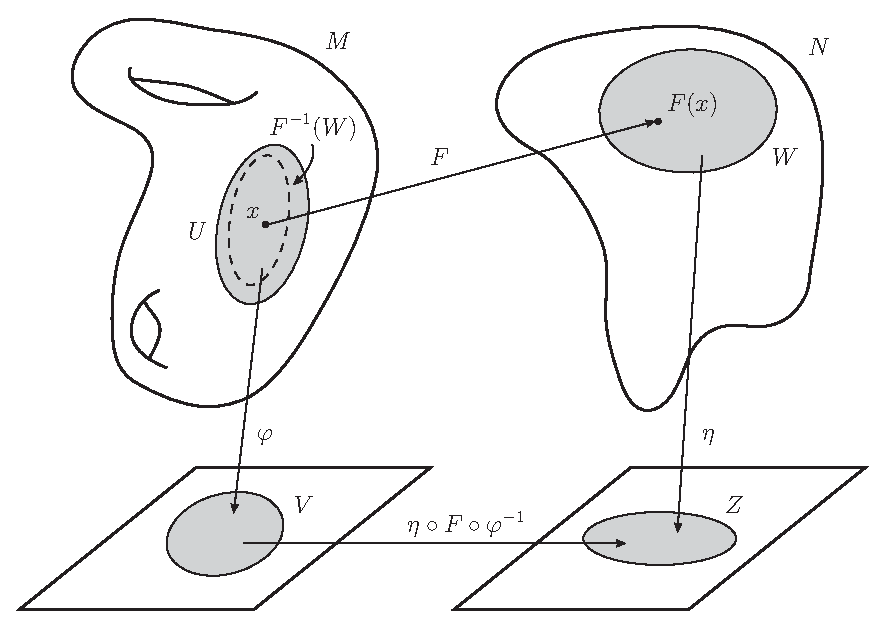
\includegraphics[scale=0.7]{fig/mani-map-1b}
\caption{A map between manifolds.}
\label{fig:mani-map-1}
\end{figure}

\subsubsection{Submanifolds}
%\texttt{Maybe use different definition?}
\begin{definition}
A subset $M$ of $\mathbb{R}^n$ is a $k$-dimensional \textit{submanifold} if for all points $x\in M$, there exists a neighbourhood $V$ of $x\in\mathbb{R}^n$, an open set $U\subseteq\mathbb{R}^k$ and a smooth map $\xi:U\to\mathbb{R}^n$ such that $\xi$ is a homeomorphism onto $M\cap V$ and $D_y\xi$ is injective for all $y\in U$. 
\end{definition}
Even though we have not yet explicitly defined what we mean by the differential of a map, $D_y\xi$, the last statement in the above definition can be interpreted as requiring continuity with respect to the `subspace topology' on $M$ induced from the inclusion into $\mathbb{R}^n$. Since open sets in the subspace topology are given by restrictions of open sets in $\mathbb{R}^n$, this is equivalent to the statement that given any open set $A\subseteq U$, there is an open set $B\subseteq\mathbb{R}^n$, such that $\xi(A)=M\cap B$.
\subsection{Tangent Spaces}
%Talk for a bit...

In this section we will give three different ways of thinking about the tangent space to a point of an abstract manifold and then show that these three characterisations are in fact equivalent.

Let $M$ be a smooth $n$-dimensional manifold. The first characterisation goes as follows. For any $x\in M$, define $T_xM$ to be the set of pairs $(\varphi,u)$ where $\varphi:U\to V$ is a chart in the atlas for $M$ with $x\in U$ and $u\in\mathbb{R}^n$, modulo the equivalence relation which identifies a pair $(\varphi,u)$ with a pair $(\eta,w)$ if and only if $u$ maps to $w$ under the derivative of the transition map between the two charts $\varphi$ and $\eta$,
\[
D_{\varphi(x)}(\eta\circ\varphi^{-1})(u)=w.
\]
The second characterisation comes about by considering what the idea of a `velocity vector' in a manifold could mean. Define $M_x$ to be space of smooth paths in $M$ through $x$. By smooth path through $x$ we mean a smooth map $\gamma:[a,b]\to M$, such that $\gamma(0)=x$. Now consider $M_x$ modulo the equivalence relation which identifies any two curves if they have the same derivative, i.e. 
\[
\gamma\sim\sigma\Leftrightarrow(\varphi\circ\gamma)'(0)=(\varphi\circ\sigma)'(0),
\] 
for some chart $\varphi:U\to V$ with $x\in U$. 

This idea is schematically illustrated below in Figure \ref{fig:tang-1}. 

\begin{figure}[h!]
\centering
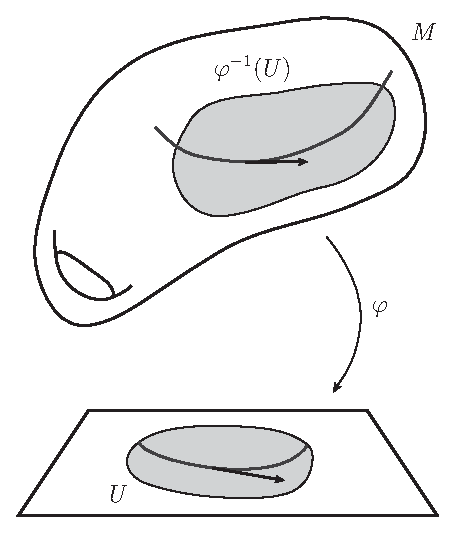
\includegraphics[scale=0.75]{fig/tang-3b}
\caption{A tangent vector to $x$ defined by a curve through $x$.}
\label{fig:tang-1}
\end{figure}

Before describing the third characterisation of tangent vectors, we have the following definition.
\begin{definition}
\label{def:derivation}
A \textit{derivation} at $x$ is a map $v:C^{\infty}(M)\to\mathbb{R}$ such that for any smooth functions $f,g$ on $M$ and real numbers $c_1,c_2$,
\begin{align*}
v(c_1f+c_2g)&=c_1v(f)+c_2v(g)\\
v(fg)&=f(x)v(g)+g(x)v(f).
\end{align*}
The first condition is simply that $v$ is linear and the second condition is known as the Leibniz identity.
\end{definition}
One of the most common examples of a derivation is the directional derivative of a function along a curve. Given a smooth path $\gamma:[a,b]\to M$ with $\gamma(0)=x$, we can compute,
\begin{equation}
v(f)=\left.\frac{d}{dt}(f\circ\gamma)\,\right\rvert_{t=0},
\label{eq:derivation-dirderiv}
\end{equation}
which defines a derivation at $x$. We can then define $D_xM$ as the space of all derivations through $x$, which is the third characterisation of the tangent space at $x$.

As stated at the beginning of the section, we can show that these three definitions of the tangent space of a point in $M$ are in fact equivalent.
\begin{proposition}
There are natural isomorphisms between the three spaces $M_x$, $T_xM$ and $D_xM$.
\[
\begin{tikzcd}[column sep=small]
T_xM \arrow{rr}{\alpha} && M_x\arrow{dl}{\beta}\\
&D_xM\arrow{ul}{\chi}
\end{tikzcd}
\]
\end{proposition}
\begin{proof}
First, given an equivalence class $[(\varphi,u)]$ in $T_xM$, take $\alpha([(\varphi,u)])$ to be the equivalence class of the smooth path given by
\[
\gamma(t)=\varphi^{-1}(\varphi(x)+tu).
\]
We have that $\alpha$ is well-defined, since if $(\eta,w)$ is another representative of the same equivalence class in $T_xM$, then $\alpha$ gives the equivalence class of the curve $\sigma(t)=\eta^{-1}(\eta(x)+tw)$ and we get,
\begin{align*}
(\varphi\circ\sigma)'(0)&=\left((\varphi\circ\eta^{-1})\circ(\eta\circ\sigma) \right)'(0)\\
&=D_{\eta(x)}\left(\varphi\circ\eta^{-1} \right)(\eta\circ\sigma)'(0)\\
&=D_{\eta(x)}\left(\varphi\circ\eta^{-1}\right)(w)\\
&=u\\
&=(\varphi\circ\gamma)'(0),
\end{align*}
and so $[\sigma]=[\gamma]$.

Now, given some $[\gamma]\in M_x$, take $\beta([\gamma])$ to be the natural derivation $v$ given by \eqref{eq:derivation-dirderiv}. We check this is well-defined as follows. Suppose $[\sigma]=[\gamma]$ and $f$ is some smooth function. Then we have,
\begin{align*}
\left.\frac{d}{dt}(f\circ\gamma)\,\right\rvert_{t=0}&=\left.\frac{d}{dt}\left[(f\circ\varphi^{-1})\circ(\varphi\circ\gamma) \right]\right\rvert_{t=0}\\
&=D_{\varphi(x)}(f\circ\varphi^{-1})(\varphi\circ\gamma)'(0)\\
&=D_{\varphi(x)}(f\circ\varphi^{-1})(\varphi\circ\sigma)'(0)\\
&=\left.\frac{d}{dt}(f\circ\sigma)\,\right\rvert_{t=0},
\end{align*}
as required.

Next, given some derivation $v$, choose a chart $\varphi$ containing $x$ and take $\chi(v)$ to be the element of $T_xM$ given by taking the equivalence class $[(\varphi,u)]$ such that $u=\left(v(\varphi^1),\ldots,v(\varphi^n)\right)$, where $\varphi^i$ is the $i$th component function of the chart $\varphi$.\\

Note the following technicality. Definition \ref{def:derivation} says that derivations must act on smooth functions defined on all of $M$, but the $\varphi^i$ are only defined on an open set $U$ of $M$. This issue is addressed by extending the $\varphi^i$ to give a smooth map defined on all of $M$. Let us define the following functions.
\begin{equation}
\xi(z)=\begin{cases}
\exp(\frac{1}{z^2-1}) & |z|<1\\
0 & |z|\geq 1
\end{cases},
\label{eq:bumpf-1}
\end{equation}
and
\begin{equation}
\rho(z)=\frac{\int_{-1}^z\xi(t)\,dt}{\int_{-1}^{1}\xi(t)\,dt}.
\label{eq:rampf-1}
\end{equation}
We have that $\xi$ is a smooth function of all of $\mathbb{R}$, with $\xi(z)>0$ on the interval $(-1,1)$ and zero otherwise. In addition, $\rho$ is a smooth function on all of $\mathbb{R}$ which is zero for $z\leq -1$, strictly increasing on the interval $(-1,1)$ and precisely one for $z>1$.

\begin{figure}[h!]
\centering
\begin{subfigure}[b]{0.5\textwidth}
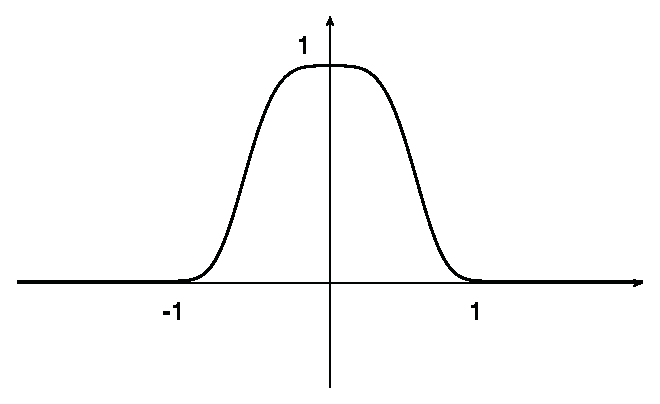
\includegraphics[scale=0.55]{fig/bump-1c}
\caption{A smooth `bump' function $\xi$.}
\end{subfigure}%
\begin{subfigure}[b]{0.5\textwidth}
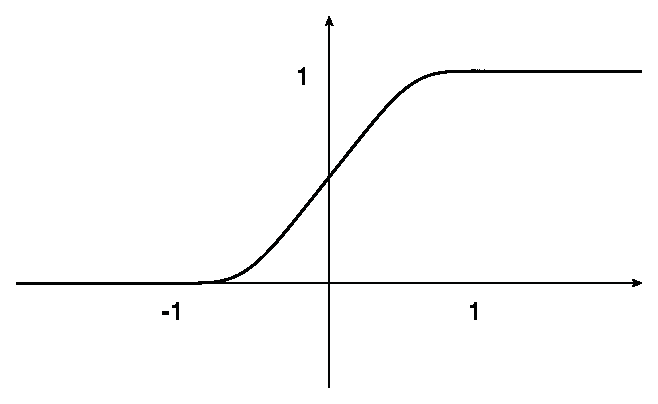
\includegraphics[scale=0.55]{fig/ramp-1c}
\caption{A smooth `ramp' function $\rho$.}
\end{subfigure}
\caption{Graphs of the functions defined by $\xi$ and $\rho$ respectively.}
\label{fig:bump-n-ramp}
\end{figure}

Given a chart $\varphi:U\to V$ with $x\in U$, choose some $\varepsilon$ sufficiently small enough to ensure that the closed ball of radius $4\varepsilon$ about $\varphi(x)$ is contained in $V$. Then define $\tilde{\rho}$ on $M$ by
\begin{equation}
\tilde{\rho}(y)=\begin{cases}
\rho\left( 3-\frac{|\varphi(y)-\varphi(x)|}{\varepsilon} \right) & y\in U,\\
0 & y\in M\backslash U.
\end{cases}
\label{eq:tilde-rho}
\end{equation}
This construction gives a function $\tilde{\rho}$ which is identically equal to one on a neighbourhood of $x$ and identically zero in the complement of a larger neighbourhood.\\

If $f:U\to\mathbb{R}$ is a smooth function on an open set $U$ of $M$ containing $x$, define $v(f)=v(\tilde{f})$ where $\tilde{f}$ is any smooth function on $M$ which agrees with $f$ on a neighbourhood of $x$.\\

We check that such a smooth function $\tilde{f}$ on $M$ which agrees with $f$ on a neighbourhood of $x$ does not depend on which function we choose as follows.

Without loss of generality, suppose $f$ is defined on $U$ as before and define $\tilde{\rho}$ as per \eqref{eq:tilde-rho}. Then define,
\begin{equation}
\tilde{f}(y)=\begin{cases}
f(y)\tilde{\rho}(y) & y\in U\\
0 & y\in M\backslash U
\end{cases},
\end{equation}
which is smooth and agrees with $f$ on the set $\varphi^{-1}\left( B_{2\varepsilon}(\varphi(x)) \right)$.\\

We verify that $v(\tilde{f})$ does not change if we choose a different function agreeing with $f$ on a neighbourhood of $x$.
\begin{lemma}
Let $f,g$ be two smooth functions on $M$ which agree on a neighbourhood of $x$. Then $v(f)=v(g)$.
\end{lemma}
\begin{proof}
Without loss of generality, suppose that $f$ and $g$ agree on an open set $U$ containing $x$ and construct a bump function $\tilde{\rho}$ in $U$ as before. Observe that $\tilde{\rho}(f-g)$ is identically zero on $M$ and that $v(0)=v(0\cdot 0)=0\cdot v(0)=0$. Hence, we have,
\[
0=v(\tilde{\rho}(f-g))=\tilde{\rho}(x)v(f-g)+(f(x)-g(x))v(\tilde{\rho})=v(f)-v(g),
\]
since $f(x)-g(x)=0$ and $\tilde{\rho}(x)=1$.
\end{proof}
Thus, the posited definition of $v(f)$ has been shown to be consistent with the definition of $\chi(v)$, and is hence is well defined. However, it remains to be checked that $\chi(v)$ is independent of our choice of a chart $\varphi$. Suppose we have another chart $\eta$. Then in a small region about $x$,
\begin{equation}
\eta^i(y)=\eta^i(x)+\sum_{j=1}^nG^i_j(y)\left( \varphi^j(y)-\varphi^j(x) \right),
\end{equation} 
for $i=1,\ldots,n$ and where $G^i_j$ is a smooth function on a neighbourhood of $x$ such that
\[
G^i_j(x)=\frac{\partial}{\partial x^j}\left.\left(\eta^i\circ\varphi^{-1}\right)\,\right\rvert_{\varphi(x)}.
\]
%\texttt{Details needed?}

Applying $v$ to $\eta^i$ yields,
\begin{align*}
v(\eta^i)&=\sum_{j=1}^n G^i_j(x)v(\varphi^j)+(\varphi^j(x)-\varphi^i(x))v(G^i_j)\\
&=\sum_{j=1}^{n}\frac{\partial}{\partial x^j}\left.\left(\eta^i\circ\varphi^{-1}\right)\,\right\rvert_{\varphi(x)}v(\varphi^j).
\end{align*}
We hence have,
\begin{align*}
\sum_{i=1}^n v(\eta^i)e_i&=\sum_{i,j=1}^n\frac{\partial}{\partial x^j}\left.\left(\eta^i\circ\varphi^{-1}\right)\,\right\rvert_{\varphi(x)}v(\varphi^j)e_i\\
&=D_{\varphi(x)}(\eta\circ\varphi^{-1})\left( \sum_{i=1}^nv(\varphi^i)e_i \right),
\end{align*}
and so $\left[ (\varphi,\sum_{i=1}^nv(\varphi^i)e_i )\right]=\left[(\eta,\sum_{i=1}^nv(\eta^i)e_i) \right]$. Thus $\chi$ is independent of the choice of chart.

It now suffices to show that $\chi\circ\beta\circ\alpha$, $\alpha\circ\chi\circ\beta$ and $\beta\circ\alpha\circ\chi$ all give the identity map on each of the three spaces.

We have the following.
\begin{align*}
\chi\circ\beta\circ\alpha([(\varphi,u)])&=\chi\circ\beta\left(\left[t\mapsto\varphi^{-1}(\varphi(x)+tu) \right] \right)\\
&=\chi\left(f\mapsto D_{\varphi(x)}(f\circ\varphi^{-1})(u) \right)\\
&=\left[ \left( \varphi,\sum_{i=1}^{n}D_{\varphi(x)}(\varphi^i\circ\varphi^{-1})(u)e_i \right) \right]\\
&=[(\varphi,u)].
\end{align*}
Next we have,
\begin{align*}
\alpha\circ\chi\circ\beta([\sigma])&=\alpha\circ\chi\left(f\mapsto\left.\frac{d}{dt}(f\circ\gamma)\,\right\rvert_{t=0} \right)\\
&=\alpha\left( \left[ \left( \varphi,\sum_{i=1}^{n}(\varphi\circ\gamma)'(0) \right) \right] \right)\\
&=\left[t\mapsto\varphi^{-1}(\varphi(x)+t(\varphi\circ\gamma)'(0)) \right],
\end{align*}
which is a curve in the same equivalence class as $\gamma$.

Finally,
\begin{align*}
\beta\circ\alpha\circ\chi(v)&=\beta\circ\alpha\left( \left[ \left( \varphi,\sum_{i=1}^{n}v(\varphi^i)e_i \right) \right] \right)\\
&=\beta\left( \left[ t\mapsto \varphi^{-1}\left( \varphi(x)+t\sum_{i=1}^nv(\varphi^i)e_i \right) \right] \right)\\
&=\left( f\mapsto\sum_{i=1}^n\frac{\partial}{\partial x^i}\left.(f\circ\varphi^{-1})\,\right\rvert_{\varphi(x)}v(\varphi^i) \right).
\end{align*}
To show that this is the same as $v$ as we require, consider the following result. Via a Taylor expansion for $f\circ\varphi^{-1}$, we have that
\[
f(y)=f(x)+\sum_{i=1}^nG_i(y)\left(\varphi^i(y)-\varphi^i(x)\right),
\]
for $y$ in a sufficiently small neighbourhood of $x$ and where $G_i$ is a smooth function such that $G_i(x)=\frac{\partial}{\partial x^i}\left. (f\circ\varphi^{-1})\,\right\rvert_{\varphi(x)}$. Applying $v$ to this expression yields,
\begin{equation}
v(f)=\sum_{i=1}^{n}G_i(x)v(\varphi^i)=\sum_{i=1}^n\frac{\partial}{\partial x^i}\left.(f\circ\varphi^{-1})\,\right\rvert_{\varphi(x)}v(\varphi^i),
\label{eq:vf-detail-1}
\end{equation}
the right hand side of which is the same as $\beta\circ\alpha\circ\chi(v)$, as required.
%\begin{center}
%\texttt{Details to be filled in...}
%\end{center}
\end{proof}
Having now established the equivalence of $M_x$, $T_x$ and $D_xM$, we shall now simply use the notation $T_xM$ to refer to the tangent space to $x$ at $M$ while using any of the three different characterisations of a tangent vector depending on what best suits the task at hand.
\subsubsection{The Differential of a Map}
\begin{definition}
Let $f:M\to\mathbb{R}$ be a smooth function. We define the differential $d_xf$ of $f$ at the point $x\in M$ to be the linear function on $T_xM$ given by $(d_xf)(v)=v(f)$ for all $v\in T_xM$, where we are considering $v$ as a derivation. 

%Let $F:M\to N$ be a smooth map between manifolds. Define the differential $D_xF$ of $F$ at $x\in M$ to be the linear map from $T_xM$ to $T_{F(x)}N$ given by $\left((d_xF)(v) \right)(f)=v(f\circ F)$ for any $v\in T_xM$ and $f\in C^{\infty}(M)$.
Let $F:M\to N$ be a smooth map between manifolds $M$ and $N$. For all points $x\in M$, define the map
\[
D_xF:T_xM\to T_{F(x)}N,
\]
to be the \textit{differential of $F$ at $x$} as follows. Given a tangent vector $v\in T_xM$, let $D_xF(v)$ be the derivation at $F(x)$ that acts on $f\in C^{\infty}(N)$ by the rule
\[
D_xF(v)(f)=v(f\circ F).
\]
\end{definition}
Alternatively, if one thinks of a vector $v$ as the tangent vector to a curve $\gamma$, then we have
\[
D_xF(v)=(F\circ\gamma)'(0),
\] 
for any smooth curve $\gamma$ such that $\gamma(0)=x$ and $\gamma'(0)=v$.
%\texttt{More detail needed?}

\begin{figure}[h!]
\centering
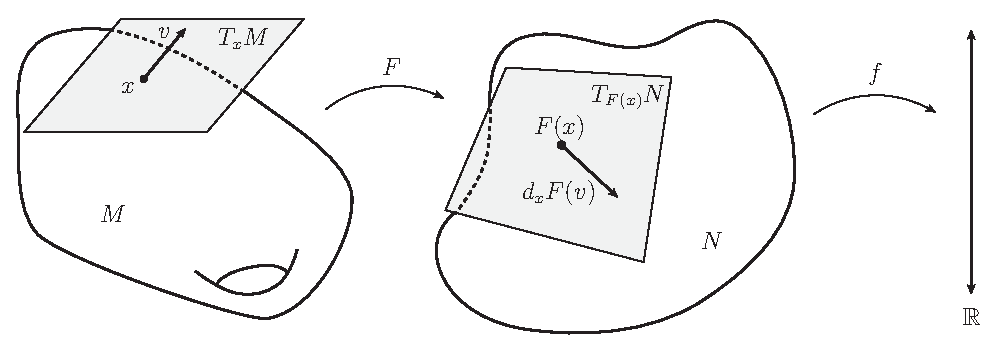
\includegraphics[scale=0.75]{fig/differential-1b}
\caption{The differential of a map $F:M\to N$.}
\label{fig:diff-1}
\end{figure}
\begin{definition}
If $F:M\to N$ is a smooth map, a point $x\in M$ is said to be a \textit{regular point of $F$} if $D_xF:T_xM\to T_{F(x)}N$ is surjective. A point $y\in N$ is said to be a \textit{regular value of $F$} is every point of the preimage $F^{-1}(y)$ is a regular point.
\end{definition}
%$v:f\mapsto (f\circ\gamma)'(0)$ and so the differential of a map $F:M\to N$ is given by the assignment,
%\[
%d_xF(v):f\mapsto (f\circ F\circ\gamma)'(0),
%\] 
%which is the tangent vector of the curve $F\circ \gamma$. This is then to say,
%\[
%d_xF([\gamma])=[F\circ\gamma].
%\]
\subsubsection{Coordinate Tangent Vectors}
We now consider how computations with tangent vectors and differentials can be carried out in local coordinates.

Let $\varphi:U\to V$ be a chart on a smooth manifold $M$ with $x\in U$. One can construct a basis for $T_xM$ by simply taking the vectors corresponding to the equivalence classes $[(\varphi,e_i)]$, where $e_1,\ldots,e_n$ are the standard basis vectors in $\mathbb{R}^n$. 

We shall adopt the notation $\partial_i=[(\varphi,e_i)]$, without explicitly referring to a chart $\varphi$. Considering this as a derivation, we have that $\partial_if=\left.\frac{\partial}{\partial x^i}(f\circ\varphi^{-1})\right\rvert_{\varphi(x)}$. This is to say, $\partial_i$ is simply the derivation given by taking the $i$th partial derivative in the coordinates defined by $\varphi$. By Proposition 2.2, it follows that $\{\partial_1,\ldots,\partial_n\}$ is a basis for $T_xM$.
%\texttt{The differential in coordinates?}
\subsection{Vector Bundles}
%\texttt{Where to put this section...}
\begin{definition}
A real \textit{vector bundle} of rank $k$ is a triple $(M,E,\pi)$. Where $M$ is a smooth manifold called the base space, $E$ is a smooth manifold called the total space and $\pi:E\to M$ is a smooth surjection called the projection. We also impose the following conditions on $\pi$.
\begin{enumerate}[(i)]
\item For all points $x\in M$, the fibre $E_x=\pi^{-1}(x)$ over $x$ is endowed with the structure of a $k$-dimensional vector space.
\item For all $x\in M$, there exists a neighbourhood $U$ of $x$ in $M$ and a homeomorphism $\psi:\pi^{-1}(U)\to U\times\mathbb{R}^k$, called the \textit{local trivialisation of $E$ over $U$}, such that:
\begin{itemize}
\item $\pi_U\circ\psi=\pi$ where $\pi_U:U\times\mathbb{R}^k\to U$ is the projection;
\item for all $q\in U$, the restriction of $\psi$ to $E_q$ is a vector space isomorphism from $E_q$ to $\{q\}\times\mathbb{R}^k\cong\mathbb{R}^k$.
\item on the intersection $U\cap V$ we have
\[
\psi_U\psi^{-1}_V:U\cap V\times\mathbb{R}^k\to U\cap V\times\mathbb{R}^k,
\]
is of the form,
\[
(x,v)\mapsto\left(x,g_{UV}(x)v\right),
\]
where $g_{UV}:U\cap V\to\mathrm{GL}(k)$.
\end{itemize}
\end{enumerate}
In an abuse of notation, we will often simply refer to a vector bundle by the map $\pi:E\to M$ since it references all elements of the formal triple $(E,M,\pi)$. 
\end{definition}

Figure \ref{fig:bundle-1} illustrates the basic concept of a vector bundle, highlighting a local trivialisation.

\begin{figure}[h!]
\centering
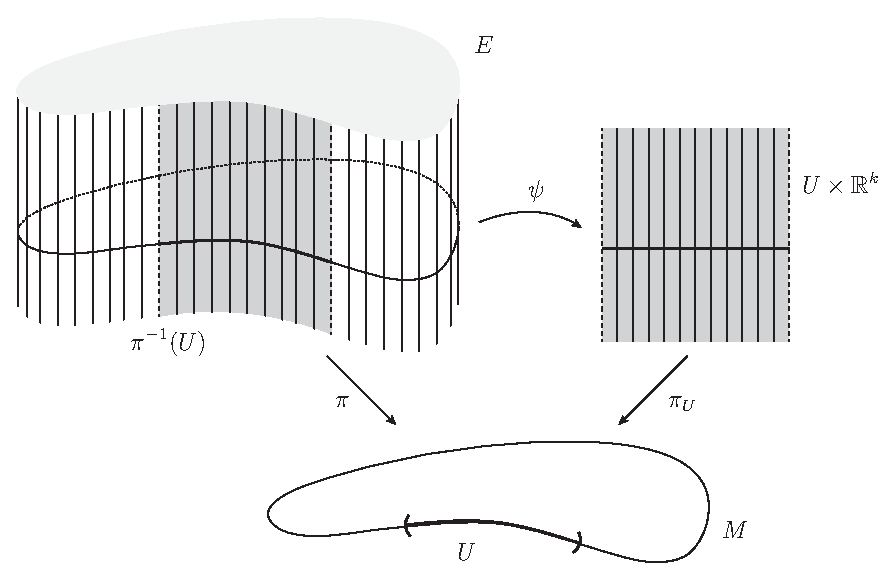
\includegraphics[scale=0.75]{fig/bundle-2b}
\caption{Sketch of a vector bundle.}
\label{fig:bundle-1}
\end{figure}

\begin{definition}
A \textit{section} of a vector bundle $\pi:E\to M$ is a continuous map $\sigma:M\to E$ satisfying $\pi\circ\sigma=\mathrm{id}_M$. This is to say that, $\sigma(x)$ is an element of the fibre $E_x$, for all points $x\in M$. A \textit{local section} is a section $\sigma$ defined on some open subset $U\subset M$. If $U=M$ then $\sigma$ is sometimes referred to as a \textit{global section}.
\end{definition}

\begin{figure}[h!]
\centering
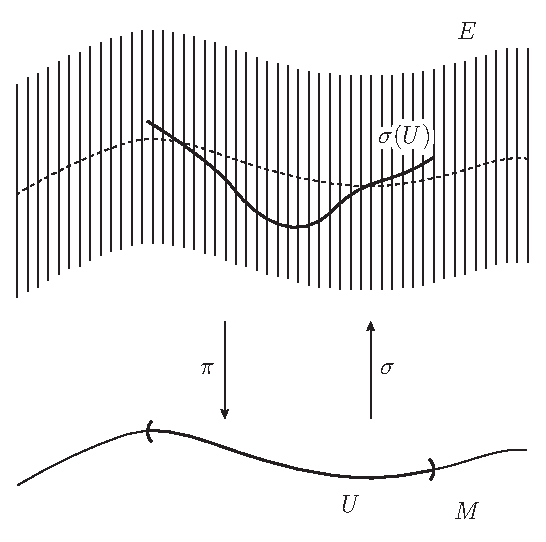
\includegraphics[scale=0.75]{fig/section-1}
\caption{Diagram illustrating a section of a vector bundle.}
\label{fig:section-1}
\end{figure}

\subsubsection{The Tangent Bundle}
It is often useful to consider the set of all tangent spaces to all points of a manifold. As such, we now consider a concrete example of a vector bundle which is of fundamental importance for this project, this being the tangent bundle of a manifold.

\pagebreak

\begin{definition}
The \textit{tangent bundle} of a manifold $M$, denoted by $TM$, is the disjoint union of the tangent spaces at all points of $M$,
\[
TM=\bigsqcup_{x\in M}T_xM=\{(x,v):x\in M,v\in T_xM\}.
\]
In terms of our definition of a vector bundle, we have $M$ as the base space, $TM$ as the total space and $\pi:TM\to M$, given by $\pi(x,v)=x$, which sends each vector in $T_xM$ to the point $x$ at which it is tangent. Furthermore, observe that
\[
(x,v)\mapsto \left(\psi\circ\varphi^{-1}(x),d(\psi\circ\varphi^{-1})v \right),
\]
gives us a vector bundle structure since $d(\psi\circ\varphi^{-1})$ is linear.
\end{definition}
If $M$ has dimension $n$, then we can endow the tangent bundle $TM$ with the structure of a $2n$-dimensional manifold. Given a chart $\varphi:U\to V$ for $M$, define a chart $\tilde{\varphi}$ for $TM$ on the set $\pi^{-1}(U)=\{(x,v)\in TM:x\in U\}$ by,
\[
\tilde{\varphi}(x,v)=\left(\varphi(x),v(\varphi^1),\ldots,v(\varphi^n) \right)\in\mathbb{R}^{2n}.
\]
The first $n$ coordinates describe the point $x$ and the last $n$ given the components of the vector $v$ with respect to the basis of the coordinate tangent vector $\{\partial_i\}_{i=1}^{n}$. From Equation \eqref{eq:vf-detail-1}, we have the following description of the local coordinate expression for $v$,
\[
v(f)=\sum_{i=1}^n\frac{\partial}{\partial x^i}\left.\left(f\circ\varphi^{-1}\right)\,\right\rvert_{\varphi(x)}v(\varphi^i)=\sum_{i=1}^nv(\varphi^i)\partial_i(f),
\]
with $f\in C^{\infty}(M)$. Hence we can write $v=\sum_{i=1}^nv(\varphi^i)\partial_i$.

To show that these charts give $TM$ a manifold structure, it suffices to compute the transition maps. Refer to \cite{MR2954043} for the explicit computation of this.

%Suppose we are given two charts $\varphi:U\to V$ and $\eta:W\to Z$ such that their intersection is non-empty.
%\begin{center}
%\texttt{Details to be filled in...}
%\end{center}

\begin{definition}[Bundle Morphism]
If $\pi:E\to M$ and $\pi':E'\to M'$ are vector bundles, a continuous map $F:E\to E'$ is a \textit{bundle morphism} (or \textit{bundle homomorphism}), if there exists a map $f:M\to M'$ such that $f\circ\pi=\pi'\circ F$,
\[
\begin{tikzcd}
E \arrow[r,"F"] \arrow{d}[swap]{\pi}
& E' \arrow[d,"\pi'"] \\
M \arrow{r}[swap]{f} & M'
\end{tikzcd}
\]
with the property that for all $x\in M$, the restricted map $F\rvert_{E_x}:E_x\to E'_{f(x)}$ is linear.

A bijective bundle homomorphism $F:E\to E'$ whose inverse is also a bundle homomorphism is called a \textit{bundle isomorphism}.
\end{definition}

\begin{example}
If $F:M\to N$ is a smooth map between manifolds $M$ and $N$ then the global differential $dF:TM\to TN$ is a smooth bundle homomorphism.
\end{example}

Let $\pi:E\to M$ be a vector bundle. If $U\subseteq M$ is an open subset, a $k$-tuple of local section $(\sigma_1,\ldots,\sigma_k)$ of $E$ over $U$ is linearly independent if $(\sigma_1(x),\ldots,\sigma_k(x))$ is linearly independent $k$-tuple in $E_x$ for all $x\in U$. Similarly, they are said to span $E$ if their values span $E_x$ for all $x\in U$.

\begin{definition}
A \textit{local frame} for $E$ over $U$ is an ordered $k$-tuple $(\sigma_1,\ldots,\sigma_k)$ of linearly independent local sections over $U$ that span $E$, i.e. $(\sigma_1(x),\ldots,\sigma_k(x))$ is a basis for the fibre $E_x$ for each $x\in U$.

If $U=M$ then it is said to be a \textit{global frame}.
\end{definition}
\begin{example}
Let $E:M\times\mathbb{R}^n\to M$ be a vector bundle. The standard basis $(e_1,\ldots,e_n)$ for $\mathbb{R}^n$ yields a global frame $(\tilde{e}_i)$ for $E$ given by $(\tilde{e}_i)(x)=(x,e_i)$.
\end{example}
\begin{example}
Let $\pi:E\to M$ be a vector bundle. If $\phi:\pi^{-1}(U)\to U\times \mathbb{R}^n$ is a local trivialisation of $E$, we can use the same technique as in the previous example to construct a local frame for $E$ over $U$. Define maps $\sigma_1,\ldots,\sigma_n: U\to E$ by $\sigma_i(x)=\phi^{-1}(x,e_i)=\phi^{-1}\circ\tilde{e}_i(x)$,
\[
\begin{tikzcd}[column sep=small]
\pi^{-1}(U) \arrow{dr}{\pi} \arrow{rr}{\phi} && U\times\mathbb{R}^n \arrow{dl}[swap]{\pi_1}\\
&U \arrow[ul, bend left, "\sigma_i"] \arrow[ur, bend right,swap,"\tilde{e}_i"]
\end{tikzcd}.
\]

The fact that $\pi_1\circ\phi=\pi$ implies that,
\[
\pi\circ\sigma_i(x)=\pi\circ\phi^{-1}(x,e_i)=\pi_1(x,e_i)=x,
\]
and so $\sigma_i$ is a section.

To see that $(\sigma_i(x))$ forms a basis for $E_x$, observe that $\phi$ restricts to an isomorphism from $E_x$ to $\{x\}\times\mathbb{R}^n$ and $\phi(\sigma_i(x))=(x,e_i)$, so $\phi$ takes $(\sigma_i(x))$ to the standard basis for $\{x\}\times\mathbb{R}^n\cong\mathbb{R}^n$.
\end{example}
In the above example, we say that the local frame $(\sigma_i)$ is \textit{associated with $\phi$}.
\begin{proposition}
Every local frame for a vector bundle is associated with a local trivialisation.
\label{vb-lf-lt}
\end{proposition}
\begin{proof}
Suppose $\pi:E\to M$ is a vector bundle and $(\sigma_i)$ is a local frame for $E$ over some open subset $U\subseteq M$. Define a map $\psi:U\times\mathbb{R}^n\to\pi^{-1}(U)$ by
\[
\psi(x,(v^1,\ldots,v^n))=v^i\sigma_i(x).
\]
From the fact that $(\sigma_i(x))$ forms a basis for $E_x$ at each point $x\in U$, we get that $\psi$ is bijective and furthermore that $\sigma_i=\psi\circ\tilde{e}_i$. Hence, if we show that $\psi$ is a diffeomorphism, then $\psi^{-1}$ will be a local trivialisation whose associated local frame is $(\sigma_i)$.

Since $\psi$ is bijective, it suffices to show that it is a local diffeomorphism. Given $y\in U$, we can find a neighbourhood $V$ of $x$ in $M$ over which there exists a local trivialisation $\phi:\pi^{-1}(V)\to V\times\mathbb{R}^n$ and by scaling $V$ if necessary, we may assume that $V\subseteq U$. Since $\phi$ is a diffeomorphism, if we show that $\phi\circ\psi\rvert_{V\times\mathbb{R}^n}$ is a diffeomorphism from $V\times\mathbb{R}^n$ to itself, it follows that $\psi$ restricts to a diffeomorphism from $V\times\mathbb{R}^n$ to $\pi^{-1}(V)$, as shown in the following diagram.
\[
\begin{tikzcd}
V\times\mathbb{R}^n\arrow{dr}[swap]{\pi_1} \arrow{r}{\psi\rvert_{V\times\mathbb{R}^n}} & \pi^{-1}(V) \arrow{r}{\phi} \arrow{d}{\pi} & V\times\mathbb{R}^n \arrow{dl}{\pi_1}\\
& V
\end{tikzcd}
\]
For each of the smooth sections $\sigma_i$, the composite map $\phi\circ\sigma_i\rvert_V:V\to V\times\mathbb{R}^n$ is smooth and hence there are smooth functions $\sigma^1_i,\ldots,\sigma^n_i:V\to\mathbb{R}$ such that
\[
\phi\circ\sigma_i(x)=\left(x,\left(\sigma^1_i(x),\ldots,\sigma^n_i(x) \right) \right).
\]
Thus, on $V\times\mathbb{R}^n$ we have,
\[
\varphi\circ\psi\left(x,(v^1,\ldots,v^n) \right)=\left(x,\left(v^i\sigma^1_i(x),\ldots,v^i\sigma^n_i(x) \right) \right),
\]
which is a composition of smooth functions and so is itself smooth.

To show $(\phi\circ\psi)^{-1}$ is smooth, note that the matrix $(\sigma^j_i(x))$ is invertible for all $x$ since $(\sigma_i(x))$ is a basis for $E_x$. Let $(\tau^j_i(x))$ denote the inverse matrix. Since matrix inversion is a smooth map from $\mathrm{GL}(n,\mathbb{R})$ to itself, the functions $\tau^j_i$ are smooth. It follows from the above computations that
\[
(\phi\circ\psi)^{-1}\left(x,(w^1,\ldots,w^n)\right)=\left(x,\left(w^i\tau^1_i(x),\ldots,w^i\tau^n_i(x) \right) \right),
\]
is a smooth function which completes the proof.
\end{proof}
\begin{corollary}
A vector bundle is trivial if and only if it admits a global frame.
\end{corollary}
\begin{proof}
From the previous examples and Proposition \ref{vb-lf-lt}, we have that there is a local trivialisation over an open subset $U\subseteq M$ if and only if there is a local frame over $U$. The corollary is simply the special case of Proposition \ref{vb-lf-lt} when $U=M$.
\end{proof}
\pagebreak
\subsection{Vector Fields}
\begin{definition}
If $M$ is a smooth manifold, a \textit{vector field on $M$} is a section of the tangent bundle, $X:M\to TM$. By definition of a section, if $\pi:TM\to M$ is the natural projection map of the tangent bundle, then
\[
\pi\circ X=\mathrm{id}_M.
\] 
In local coordinates we have,
\[
X(x_1,\ldots,x_n)=(x_1,\ldots,x_n,X^1(x),\ldots,X^n(x)),
\]
where the $X^i(x)$ are smooth functions. Hence the tangent vector $X(x)$ is given by,
\begin{equation}
X_x=\sum_iX^i(x)\left(\frac{\partial}{\partial x^i}\right)_x,
\label{eq:vect-local}
\end{equation}
which is a smoothly varying field of tangent vectors.
\end{definition}
From our definition of tangent vectors in terms of derivations, we also have the following proposition which allows us to describe vector fields in terms of derivations.
\begin{proposition}
Let $X:C^{\infty}(M)\to C^{\infty}(M)$ be a linear map which satisfies the Leibniz identity,
\[
X(fg)=f(Xg)+g(Xf).
\]
Then $X$ is a vector field.
\end{proposition}
\begin{proof}
Given such a derivation $X$ and $x\in M$, the map $X_x:C^{\infty}(M)\to\mathbb{R}$ given by $X_x(f)=(X(f))(x)$ is a derivation at $x$ and so defines an element of $T_xM$. The map $x\mapsto X_x$ from $M$ to $TM$ is hence a vector field and it remains to check smoothness. The components of $X_x$ with respect to the coordinate tangent basis $\partial_1,\ldots,\partial_n$ for a chart $\varphi:U\to V$ is given by,
\[
X_x^i=X_x(\varphi^i),
\]
which is by assumption a smooth function of $x$ for each $i$ (since $\varphi^i$ is a smooth function and $V$ maps smooth functions to smooth functions). We can extend the $\varphi^i$ by a bump function such as the one given by Equation \eqref{eq:bumpf-1} in a coordinate neighbourhood to convert it to a smooth function on the whole of $M$. Hence the vector field is smooth.

Conversely, given a smooth vector field $x\mapsto X_x\in T_xM$, the map,
\[
(X(f))(x)=X_x(f),
\] 
satisfies the conditions necessary for a derivation and takes a smooth function to a smooth function.
%For all $x\in M$, $X_x(f)$ satisfies the conditions for a tangent vector at $x$, and so $X$ defines a map $X:M\to TM$ with $\pi\circ X=\mathrm{id}_M$ and can be written locally in the form of Equation \eqref{eq:vect-local}.
%
%It suffices to show that the $y_i(x)$ are smooth, and for this we simply need to apply $X$ to a coordinate function $x_i$ extended by a bump function \texttt{should probably define this earlier on somewhere eh?} in a coordinate neighbourhood. This is simply,
%\[
%Xx_i=y_i(x),
%\]
%and since by assumption $X$ maps smooth functions to smooth functions, the $y_i(x)$ are smooth.
\end{proof}
\begin{remark}
In this report, we are interested in \textit{nowhere vanishing} vector fields on spheres. By this, it is meant that given some vector field $X$ on $\mathbb{S}^n$, we want $X(x)\neq 0$ for any given point $x\in\mathbb{S}^n$.
\end{remark}
\subsection{Differential Forms}
%\textbf{\textcolor{red}{Might have to go unused...}}\\
In order to build up to the notion of a differential form, we have the following definitions.
\begin{definition}
A \textit{covector} $\omega$ at $x\in M$ is a linear map from $T_xM$ to $\mathbb{R}$. The set of covectors at $x$ form an $n$-dimensional vector space denoted by $T^*_xM$ (in the language of linear algebra, this is the dual space to $T_xM$).
\end{definition}
\begin{definition}
A \textit{tensor} of type $(k,l)$ at $x$ is a multilinear map $T_x$ which takes $k$ vectors and $l$ covectors and returns a real number,
\[
T_x:\underbrace{T_xM\times\cdots\times T_xM}_{k\text{ copies}}\times\underbrace{T^*_xM\times\cdots\times T^*_xM}_{l\text{ copies}}\to\mathbb{R}.
\]
A tensor of type $(k,0)$ is also referred to as a \textit{covariant $k$-tensor}, while a a tensor of type $(0,l)$ is referred to as a \textit{contravariant $l$-tensor}. We denote the space of covariant $k$-tensors by $T^kT^*_xM$.
\end{definition}
We note that a covector can be seen as a tensor of type $(1,0)$ and a vector is a tensor of type $(0,1)$, since a vector $v$ acts linearly on a covector $\omega$ by $v(\omega):=\omega(v)$.\\

To get a better understanding of what this definition implies, let us work in a chart such that we have a basis of coordinate tangent vector fields $\partial_1,\ldots,\partial_n$ at each point. Then we can define a basis for the cotangent space $T^*_xM$ as,
\[
dx^i:T_xM\to\mathbb{R},
\]
where,
\[
dx^i(\partial_j)=\delta^i_j=\begin{cases}
1 & i=j\\
0 & i\neq j
\end{cases}.
\]
The notation comes from the fact that $dx^i$ is the differential of the smooth function $x^i$, i.e.
\[
dx^i(v)=v(x^i).
\]
Similarly for any smooth function $f$ on $M$, we have a covector, $d_xf\in T^*_xM$ defined by,
\[
df(v)=v(f).
\]
\begin{definition}
Let $T$ and $S$ be two tensors at $x$ of types $(k,l)$ and $(p,q)$ respectively. The \textit{tensor product} $T\otimes S$ is the tensor at $x$ of type $(k+p,l+q)$ defined by,
\begin{align*}
T\otimes S(v_1,\ldots,v_{k+p},\omega_1,\ldots\omega_{l+q})&=T\left(v_1,\ldots,v_k,w_1,\ldots,w_l \right)\\
&\times S\left(v_{k+1},\ldots,v_{k+p},w_{l+1},\ldots,w_{l+q} \right),
\end{align*}
for all vectors $v_1,\ldots,v_{k+p}\in T_xM$ and covectors $\omega_1,\ldots,\omega_{l+q}\in T^*_xM$.
\end{definition}
%\texttt{Maybe better to define it in terms of its properties instead?}
\begin{definition}
A $k$-tensor $\omega\in T^kT^*_xM$ is said to be \textit{alternating} if it is antisymmetric under interchange of any two of its arguments. Alternatively, for any $k$ vectors, $v_1,\ldots,v_k\in T_xM$ and any permutation $\sigma\in S_k$,
\[
\omega(v_{\sigma(1)},\ldots,v_{\sigma(k)})=\mathrm{sgn}(\sigma)\omega(v_1,\ldots,v_k),
\]
where,
\[
\mathrm{sgn}(\sigma)=\begin{cases}
1 & \text{if }\sigma\text{ is an even permutation},\\
-1 & \text{if }\sigma\text{ is an odd permutation}.
\end{cases}
\]
\end{definition}
The space of alternating $k$-tensors at $x$ is denoted by $\Lambda^kT^*_xM$.

There is a natural projection $\mathcal{A}:T^kT^*_xM\to\Lambda^kT^*_xM$ given by,
\[
\mathcal{A}T(v_1,\ldots,v_k)=\frac{1}{k!}\sum_{\sigma\in S_k}\mathrm{sgn}(\sigma)T(v_{\sigma(1)},\ldots,v_{\sigma(k)}).
\]
\begin{definition}
Let $S\in\Lambda^kT^*_xM$ and $T\in\Lambda^lT^*_xM$ be alternating tensors. The \textit{wedge product} $S\wedge T$ of $S$ and $T$ is the alternating $k+l$-tensor given by,
\[
S\wedge T=\frac{(k+l)!}{k!l!}\mathcal{A}(S\otimes T)
\]
\end{definition}
More often than not we are more interested in the properties of the wedge product than using the actual definition. As such, we have the following.
\begin{proposition}
The wedge product is characterised by the following properties.
\begin{enumerate}[(i)]
\item Associativity: $f\wedge(g\wedge h)=(f\wedge g)\wedge h$;
\item Homogeneity: $(cf)\wedge g=c(f\wedge g)=f\wedge(cg)$;
\item Distributivity: $(f+g)\wedge h=(f\wedge h)+(g\wedge h)$;
\item Anticommutativity: If $f\in\Lambda^kT^*_xM$ and $g\in\Lambda^l T^*_xM$, then $g\wedge f=(-1)^{kl}f\wedge g$;
\item In any given chart: \[(dx^{i_1}\wedge\cdots\wedge dx^{i_k})\wedge(dx^{j_1}\wedge\cdots\wedge dx^{j_l})=dx^{i_1}\wedge\cdots\wedge dx^{i_k}\wedge dx^{j_1}\wedge\cdots\wedge dx^{j_l} \]
\end{enumerate}
\end{proposition}
For a proof of the above proposition, see \cite{andrews}.\\

Given a basis $\{\partial_1,\ldots,\partial_n\}$ for $T_xM$, we define a natural basis for $\Lambda^kT^*_xM$ as follows. For each $k$-tuple, $i_1,\ldots,i_k$ (for $i=1,\ldots,n$), define,
\[
dx^{i_1}\wedge\cdots\wedge dx^{i_k}=k!\mathcal{A}(dx^{i_1}\otimes\cdots\otimes dx^{i_k}).
\]
It is worth noting that these `elementary' alternating $k$-tensors have quite a clear geometric interpretation. The value of $dx^I(v_1,\ldots,v_k)$ is the determinant of the matrix with the coefficient in the $(m,n)$ position given by $dx^{i_m}(v_n)$. This gives the signed $k$-dimensional volume of the projection of the parallelopiped generated by $v_1,\ldots,v_k$ onto the subspace generated by $\partial_{i_1},\ldots,\partial_{i_k}$.\\

As with tangent and cotangent spaces, we may form the bundle of alternating $k$-tensors on $M$ and as one may expect, it is given by,
\[
\Lambda^kT^*M=\bigcup_{x\in M}\Lambda^kT^*_xM.
\]  
This is a vector bundle and hence also has the structure of a manifold.
%\texttt{Show this?}

Since it is a vector bundle, we have the natural projection $\pi:\Lambda^kT^*M\to M$. Perhaps more importantly however, we have the following.
\begin{definition}
A \textit{differential $k$-form} $\omega$ on a smooth manifold $M$ is a smooth section of the bundle of alternating $k$-tensors on $M$. To each point $x\in M$, $\omega$ associates an alternating $k$-tensor $\omega_x$ in such a way that in any chart for $M$ the coefficients $\omega_{i_1\ldots i_k}$ are smooth functions. The space of differential $k$-forms on $M$ is denoted by $\Omega^k(M)$.
\end{definition}
In local coordinates, we may write a differential $k$-form as
\[
\omega=\sum_{i_1<\ldots<i_k}a_{i_1\ldots i_k}(x)dx^{i_1}\wedge\cdots\wedge dx^{i_k}=\sum a_I(x)dx^I,	
\]
where the $a_I(x)$ are smooth functions.
\pagebreak
\begin{proposition}
On any manifold $M$ there exists a unique linear operator $\mathrm{d}:\Omega^k(M)\to\Omega^{k+1}(M)$ called the \textit{exterior derivative} such that,
\begin{enumerate}[(i)]
\item If $f\in\Omega^0(M)=C^{\infty}(M)$, then $\mathrm{d}f$ agrees with the differential of $f$;
\item If $\omega\in\Omega^k(M)$ and $\eta\in\Omega^l(M)$, then
\[
\mathrm{d}(\omega\wedge\eta)=(\mathrm{d}\omega)\wedge\eta+(-1)^k\omega\wedge(\mathrm{d}\eta);
\]
\item $\mathrm{d}^2=0$.
\end{enumerate}
\end{proposition}
For a proof see \cite{andrews}.\\

%\subsubsection{Stokes' Theorem}
\begin{theorem}[Stokes' Theorem]
Let $M$ be a compact $n$-dimensional differentiable manifold with boundary and let $\omega\in\Omega^{n-1}(M)$. Then
\[
\int_M\,d\omega=\int_{\partial M}\omega.
\]
\label{thm:stokes}
\end{theorem}
\begin{proof}
Refer to \cite{andrews}.
\end{proof}
%\subsubsection{Gauss-Bonnet \& Poincar\'{e}-Hopf}
%\subsection{Result 1?}
%asdf
%\subsection{Hopf Maps}
%asdf
%\subsection{Result 2?}
%asdf
\subsection{Parallelisability}
\begin{definition}
A smooth, $n$-dimensional manifold $M$ is said to be \textit{parallelisable} if and only if its tangent bundle $TM$ is trivial, i.e. $TM$ is isomorphic to $M\times\mathbb{R}^n$.
\end{definition}
\begin{proposition}
A smooth, $n$-dimensional manifold $M$ is parallelisable if and only if there exist $n$ linearly independent vector fields. In other words, there exist $X_1,\ldots X_n$ on $M$ such that $\left(X_1(x),\ldots, X_n(x) \right)$ is a basis for $T_xM$, for all points $x\in M$.
\label{prop:para-condn}
\end{proposition}
\begin{proof}
Suppose $M$ is parallelisable, then $TM\cong M\times\mathbb{R}^n$. Define the map $v_i:M\to M\times\mathbb{R}^n$ such that $x\mapsto (x,e_i)$. Clearly these maps are linearly independent at each point $x\in M$ and induce independent vector fields on $M$ by composing with the isomorphism $M\times \mathbb{R}^n\to TM$.\\

Now suppose that there are $n$ independent vector fields $\{v_1,\ldots,v_n\}$ on $M$. Then we can construct an isomorphism from $TM$ to $M\times\mathbb{R}^n$ by setting $v_i(x)\simeq (x,e_i)$ for all $x\in M$ and $i\in\{1,\ldots,n\}$.
\end{proof}
%\begin{theorem}
%Suppose $V$ is a continuous vector field on $\mathbb{S}^2$. Then there exists a point $p\in\mathbb{S}^2$ such that $V(p)=0$.
%\end{theorem}
%\begin{proof}
%tbc
%\end{proof}
%\paragraph{The Tangent Bundle}
%\hfill\\
%asdf
\pagebreak
 \section{Constructing Parallelisations}
In order to first motivate some of the results in this section, we will prove the famous Hairy Ball Theorem\footnote{Depending on the referece, this theorem may either refer to the case of all even dimensional spheres or simply the case for $\mathbb{S}^2$ - in this case we will opt for the latter characterisation.}. We will see that this is in fact a special case of a more general theorem which we will also prove. Two proofs are given, one of an analytic nature due to Milnor \cite{MR505523} and the other using the Poincar\`{e}-Hopf theorem which we prove.
We shall then construct explicit parallelisations for $\mathbb{S}^n$, $n=1,3,7$. Finally we discuss results related to the existence of division algebras.
 
\begin{proposition}
The sphere $\mathbb{S}^2$ does not admit a non-vanishing continuous tangent vector field and hence, $\mathbb{S}^2$ is not parallelisable.
\end{proposition}

%\begin{proof}
%Suppose, for a contradiction, that $\mathbb{S}^2$ does in fact admit a continuous non-vanishing vector field $V$. Since $V$ is non-vanishing we may assume that $V$ has unit length, or else renormalise, $\frac{V}{|V|}$.
%\end{proof}
%
%To prove this, we will prove the Poincar\`{e}-Hopf theorem for surfaces which will immediately imply the result.
%
Before we prove the above proposition, we have the following definitions.

\begin{definition}
A \textit{Riemannian metric} (often referred to simply as a metric; not to be confused with a distance function) $g$ on a smooth manifold $M$ is a smooth choice of inner product on each tangent space of the $M$, $g_x:T_xM\times T_xM\to\mathbb{R}$. Since $g$ is an inner product, for all $x\in M$, $g=g_x$ satisfies the following.
\begin{enumerate}
\item $g(u,v)=g(v,u)$, $\forall u,v\in T_xM$.
\item $g(u,v)\geq 0$, $\forall u\in T_xM$.
\item $g(u,v)=0$ if and only if $u=0$.
\end{enumerate}
Further, $g$ is said to be smooth in the sense that if $X,Y$ are smooth vector fields, then $x\mapsto g_x(X_x,Y_x)$ is smooth.

In local coordinates, a metric can be described in terms of its coefficients in a local chart, given by $g_{ij}=g(\partial_i,\partial_j)$. Smoothness of $g$ is equivalent to smoothness of the coefficient functions $g_{ij}$ is a given chart.
\end{definition}

%\textcolor{red}{\textbf{Connection 1-form}: Bugger, going to have to rethink this...}
\begin{definition}
An atlas $\mathcal{A}$ for a smooth manifold $M$ is \textit{orientable} if whenever charts $\varphi$ and $\eta$ in $\mathcal{A}$ have a non-trivial, common domain of definition, the Jacobian $\det(\eta\circ\varphi^{-1})$ is positive. An \textit{orientation} on an orientable manifold is an equivalence class of oriented atlases, where two oriented atlases are equivalent if their union is an oriented atlas.
\end{definition}
\begin{definition}
The \textit{Euler characteristic}, denoted by $\chi=\chi(M)$ (not to be confused with the space of all vector fields on $M$, though this should be clear from context), is a topological invariant. If $M$ admits a triangulation, (i.e. a decomposition into diffeomorphic images of closed $n$-simplices such that the intersection of any two is either empty or a common $(n-k)$-simplex ($k<n$)), then the Euler characteristic is given by
\[
\chi(M)=\sum_i(-1)^is_i,
\] 
where the $s_i$ are the number of $i$-dimensional simplices of a given triangulation of $M$.
It is a well known, though non-trivial to prove, result that every smooth manifold does admit such a triangulation \cite{whitehead1940c1}. Furthermore, if the manifold is compact then the triangulation may be chosen such that it is finite.
\end{definition}

Now, consider the following results regarding compact oriented two-dimensional manifolds.

\begin{theorem}[Gauss-Bonnet]
Let $M$ be a compact oriented two-dimensional manifold equipped with a Reimannian metric $g$. Let $K$ be the Gaussian curvature of $M$ and $k_g$ be the geodesic curvature of $\partial M$. Then,
\[
\int_MK\,dA+\int_{\partial M}k_g\,ds=2\pi\chi(M).
\] 
\end{theorem}
\begin{proof}
Refer to \cite{andrews} or \cite{guillemin2010differential}.
\end{proof}
\begin{theorem}[Poincar\'{e}-Hopf (Surfaces)]
Let $M$ be a compact oriented two-dimensional manifold. Let $V$ be any vector field on $M$ which has all zeroes isolated, that is, if $y$ is any zero of $V$ then there is a neighbourhood $U$ of $y$ in $M$ such that $V$ is non-zero on $U\backslash\{y\}$. Label the zeroes of $V$ as $x_1,\ldots,x_k$. Then 
\[\sum_{i=1}^{k}\mathrm{Ind}_x(V)=\chi(M).\]
\label{thm:poinhopf}
\end{theorem}
\begin{proof}
A proof of the generalised form of this theorem for manifolds is presented in Section \ref{sec:ph-gen-sec}.
\end{proof}
%The following proof is due to Andrews,\cite{andrews}.
%\begin{proof}
%Let $V$ and $g$ be given and let $x_1,\ldots,x_N$ be the zeroes of $V$. About each zero, choose a neighbourhood $U_i$ of $x_i$ such that $V$ is non-vanishing on $\tilde{M}=M\backslash\bigcup_{i=1}^NU_i$. Let $\gamma_i$ be the boundary of the $U_i$ parametrised anticlockwise in some oriented chart.
%
%Define $e_1=\frac{V}{g(V,V)^{1/2}}$ and take $e_2$ to be the unit vector orthogonal to $e_1$. Denote the dual frame by $\omega_1$ and $\omega_{2}$.
%\textbf{\textcolor{red}{TBC?}}
%\end{proof}
\begin{remark}
We note that since $\mathbb{S}^2$ has no `edge' the integral over $\partial\mathbb{S}^2$ is zero. Furthermore, recall that the Gaussian curvature of $\mathbb{S}^2$ with the standard metric is 1 \cite{andrews}. From Gauss-Bonnet we have that the left-hand side is non-zero and so the right-hand side must be non-zero, i.e. the Euler characteristic is non-zero. It follows by Poincar\`{e}-Hopf that any vector field $V$ on $\mathbb{S}^2$ must vanish somewhere. Thus, $\mathbb{S}^2$ is not parallelisable. 
\end{remark} 
We have the following more general result (which also immediately implies the Hairy Ball Theorem).
\begin{theorem}
\label{thm:novan-iff-odd}
The sphere $\mathbb{S}^n$ admits an everywhere non-zero smooth vector field if and only if $n$ is odd.
\end{theorem}
In order to prove this result, we will break the theorem up into two parts. Proposition \ref{prop:even-noVF} will give the necessary condition and then in Section 3.2 we will provide the sufficient condition for the theorem.
\begin{proposition}
\label{prop:even-noVF}
If $n$ is even, then there exists no nowhere vanishing smooth vector field on $\mathbb{S}^n$.
\end{proposition}
The following proof is due to Milnor \cite{MR505523} and uses only basic techniques from analysis as opposed to other proofs that make use of more algebraic methods such as (co)homology theory.
\begin{proof}
Suppose for the sake of a contradiction, that such a vector field $V:\mathbb{S}^n\to\mathbb{R}^{n+1}$ exists. Without loss of generality, we may set $\|V(x)\|=1$ for all $x$, otherwise we may simply normalise the vector since by hypothesis $\|V(x)\|\neq 0$. Let $A$ be a compact region of $\mathbb{R}^{n+1}$ given by,
\[
A=\{y\in\mathbb{R}^{n+1}:1-\varepsilon\leq\|y\|\leq 1+\varepsilon\},
\] 
for $0<\varepsilon<1$. We can expand $V$ onto $A$ by continuing linearly over the rays, i.e. set $V(x)=\|x\|V(\frac{x}{\|x\|})$. Now consider the function,
\[
f_t(x)=x+tV(x),
\]
for $t\in\mathbb{R}$ and which is defined for all $x\in A$. Furthermore, since $\langle x,V(x)\rangle=0$ for all $x\in A$, we have that $\|f_t(x)\|=\|x\|\sqrt{1+t^2}$.

We now have the following lemmas which will give us the contradiction we seek.
\begin{lemma}
For sufficiently small $t>0$, the mapping $f_t$ is one-to-one and maps the region $A$ onto a region $f_t(A)$ whose volume can be expressed as a polynomial function in $t$.
\end{lemma}
\begin{proof}
Since $A$ is compact and since $V$ is smooth, there exists a Lipschitz constant $c>0$ such that,
\[
\|V(x)-V(y)\|\leq c\|x-y\|,
\]
for all $x,y\in A$. We see this from the fact that since all the partial derivatives are continuous, by the mean value theorem from calculus, they attain a maximum on $A$ and taking the maximum of these yields $c$.

Choose $t$ such that $|t|<c^{-1}$ and suppose that $f_t(x)=f_t(y)$. Then we get $x-y=t(V(y)-V(x))$ and hence \[\|x-y\|=|t|\|V(y)-V(x)\|\leq c|t|\|x-y\|,\] and since $0<|t|c<1$, we have that $x=y$ and so $f_t$ is injective.\\

Via the change of variables theorem, we have that,
\[
\mathrm{vol}(f_t(A))=\int_{f_t(A)}1\,\mathrm{d}y=\int_A|\mathrm{det}(Df_t(x))|\,\mathrm{d}x.
\]
We note that since $Df_t(x)=I+tD\,V(x)$ (where $I$ is the identity matrix) and the determinant of a finite dimensional matrix is a polynomial in its entries, we get that \[\mathrm{det}(Df_t(x))=1+t\sigma_1(x)+\ldots+t^k\sigma_k(x),\] where the $\sigma_i$ are polynomials of all the partial derivatives of $V$ and hence continuous in $x$. Now, choosing $t$ sufficiently small, we have that $\mathrm{det}(Df_t(x))>0$ for all $x\in A$ and we have,
\begin{align*}
\mathrm{vol}(f_t(A))&=\int_A|\mathrm{det}(Df_t(x))|\,\mathrm{d}x\\
&=\int_A\mathrm{det}(Df_t(x))\,\mathrm{d}x\\
&=\int_A\sum_{i=0}^kt^i\sigma_i(x)\,\mathrm{d}x\\
&=\sum_{i=0}^kt^k\left[\int_A\sigma_i(x)\,\mathrm{d}x\right],
\end{align*}
which is clearly a polynomial function in $t$. This completes the proof of the lemma.
\end{proof}
\begin{lemma}
For sufficiently small $t>0$, the unit sphere is mapped onto the sphere of radius $\sqrt{1+t^2}$.
\end{lemma}
\begin{proof}
When $t$ is sufficiently small, such that the determinant of $Df_t(x)$ is always strictly positive and hence $Df_t(x)$ is non-singular, we have via the inverse function theorem that $f_t$ maps open sets to open sets. As such, if we restrict $f_t$ from $\mathbb{S}^n$ to the ball $B^{n+1}$ of radius $\sqrt{1+t^2}$, we have that $f_t(\mathbb{S}^n)$ is open in the larger sphere. On the other hand, since we are working in a finite dimension, $\mathbb{S}^n$ is compact and so we have that the image under $f_t$ is also compact and hence closed in the larger sphere. Since the codomain is connected, we have that the image is both open and closed in the codomain, and so it must be the entire sphere, i.e. $f_t(\mathbb{S}^n)=B^{n+1}_{\sqrt{1+t^2}}$ and the result follows. 
\end{proof}
By the second lemma, we get that $A$ is mapped onto $\{\sqrt{1+t^2}(1-\varepsilon)\leq\|x\|\leq\sqrt{1+t^2}(1+\varepsilon)\}$, which has volume $\sqrt{1+t^2}^{n+1}\mathrm{vol}(A)$. If $n$ is even, then $\sqrt{1+t^2}^{n+1}$ is not a polynomial function. Hence, we get a contradiction with lemma 1 and so our original assumption that there exists a nowhere vanishing smooth vector field on $\mathbb{S}^n$ must be incorrect.
\end{proof}
As we are about to see, this motivating example of the Hairy Ball theorem is merely a special case of the following more general result, which also acts as a stepping stone to establishing which sphere admits parallelisations.\\

\subsection{Existence of a Non-Vanishing Vector Field}
As we have seen in the previous example and theorem, even dimensional spheres do not admit even a single everywhere non-zero smooth vector field. This tells us that we must focus our study solely on odd dimensional spheres. Ultimately, we wish to establish some maximal number of independent vector fields; before this however, an important question to perhaps ask, is whether there exists even one pointwise linearly independent vector field on $\mathbb{S}^n$.

The answer to this question thankfully, is ``yes'', we can guarantee the existence of at least one nowhere vanishing smooth vector field on $\mathbb{S}^n$. If $n$ is odd, writing $n=2k-1$, the sphere $\mathbb{S}^n$ can be embedded in $\mathbb{R}^{2k}$ and we can write down the following nowhere vanishing vector field $V:\mathbb{S}^{2k-1}\to\mathbb{R}^{2k}$ given by,
\begin{equation}
V(x_1,x_2,\ldots,x_{2k-1},x_{2k})=(-x_2,x_1,\ldots,-x_{2k},x_{2k-1}).
\label{eq:novan-vect-1}
\end{equation}
Clearly, any point $x$ on the sphere is not zero and so $V(x)$ is nowhere vanishing for all points $x\in\mathbb{S}^{2k-1}$.\\

Furthermore, we have,
\[
x\in\mathbb{R}^{2k}\mapsto (x,V(x))\in\mathbb{R}^{2k}\times\mathbb{R}^{2k}=T\mathbb{R}^{2k}.
\] 
Consider the position vector field on the sphere $R$ which is given by,
\[
x\mapsto (x,x),
\]
It can be shown through a tedious but simple computation that,
\[
\langle V(x),R(x)\rangle=0.
\]
This is to say then that the vector field $V$ is orthogonal $R$, but $R$ is also the normal vector field to the sphere. So $V$ must be tangent to the sphere.\\

The construction given above together with Proposition \ref{prop:even-noVF} concludes the proof for Theorem \ref{thm:novan-iff-odd}.

\subsection{Poincar\`{e}-Hopf (General) \label{sec:ph-gen-sec}}
\begin{theorem}
Let $M$ be a compact orientable manifold, then there exists a non-vanishing vector field on $M$ if and only if $\chi(M)=0$.
\end{theorem}
We give a sketch of the proof below, many of the proofs of the lemmas stated are omitted. We refer the reader to \cite{wrightPoincare} for details.
\begin{proof}
We must first define the mapping degree of a map between orientable manifolds. Take a map $f:M\to N$ with $M,N$ compact orientable manifolds of the same dimension and take $y\in N$ a regular value of $f$. It follows that $f^{-1}(y)$ is a set of discrete points on a compact manifold and hence finite. Define the degree by
\[
\mathrm{deg}(f,y)=\sum_{x\in f^{-1}(y)}\mathrm{sign}(df)_x,
\]
where we take $\mathrm{sign}(df)_x$ to really be read as $\mathrm{sign}(\det(df)_x)$ with respect to the positively oriented basis.

We have the following lemma which will be used to show that degrees are invariant under extensions.
\begin{lemma}[Extension Lemma]
Let $M$ be an $n+1$-dimensional manifold with boundary and $N$ be an $n$-dimensional manifold. Let $f:\partial M\to N$ be a map and $y\in N$ be a regular value of $f$. If $f$ has an extension $F:M\to N$, then $\mathrm{deg}(f,y)=0$.
\end{lemma}
%\begin{proof}
%See \textbf{PoincareHopf.pdf}.
%\end{proof}
\begin{corollary}
If $g_0$ and $g_1$ are smoothly homotopic maps that have a common regular value $y$, then $\mathrm{deg}(g_0,y)=\mathrm{deg}(g_1,y)$.
\label{cor:homt-deg}
\end{corollary}
\begin{proof}
Let $G:M\times [0,1]\to N$ be a homotopy such that $G(\cdot,0)=g_0$ and $G(\cdot,1)=1$. By the previous lemma, we have that
\[
\partial(M\times [0,1])=M\times\{1\}- M\times\{0\},
\]
and so
\[
\mathrm{deg}(F\rvert_{\partial(M\times [0,1])},y)=\mathrm{deg}(g_1,y)-\mathrm{deg}(g_0,y).
\]
\end{proof}
Corollary \ref{cor:homt-deg} allows us to now talk about $\deg(f,y)$ whenever there exists a function $g$ homotopic to $f$ such that $y$ is a regular value of $g$. The consequence of this is that $y$ no longer needs to be a regular value of $f$, so long as it is a regular value of $g$. It can be shown that the existence of such a function $g$ which is homotopic to $f$ with regular value $f$ is guaranteed (see \cite{BurnsGidea,wrightPoincare}). Hence $\deg(f,\cdot)$ is defined globally.

%\begin{proposition}
%
%\end{proposition}
%
We will now define the index of a zero of a vector field, first in the setting of $\mathbb{R}^n$. Suppose we have a vector field $V:\mathbb{R}^n\to\mathbb{R}^n$ such that $V(0)=0$ and there is a closed disk $D$ around 0 such that the only zero of $V$ on $D$ is 0. Then we have a map \[u:\partial D\to\mathbb{S}^{n-1};\,\,\, u(z)=\frac{V(z)}{|V(z)|}.\] Define the index of the zero, $\mathrm{Ind}_x(V)$, as the degree of $u$.

\begin{proposition}
$\mathrm{Ind}_x(V)$ does not depend on the choice of $D$ or the choice of local coordinates
\end{proposition}
\begin{proof}
To show the first part of the claim, consider the following. Picking another disk $D'$ centered at $x$, we can find a disk $D_0$ contained in both $D$ and $D'$. The extension lemma gives us that the degrees of $u:D\to\mathbb{S}^{n-1}$ and $u_0:D_0\to\mathbb{S}^{n-1}$ are the same and by the same argument, so are the degrees of $u':D'\to\mathbb{S}^{n-1}$ and $u_0$. Hence the index does not depend on our choice of $D$.

To show that the index is independent of our choice of coordinates we refer the reader to \cite{BurnsGidea} for a detailed proof.

%Consider two local coordinate charts near a fixed point $x_0$ of a map $f:M\to M$
\end{proof}

Given a vector field with a discrete number of zeroes, we choose charts around those zeroes and use the same construction as before. Denote the index of a zero, $x$, of a vector field $V$ by $\mathrm{Ind}_x(V)$.

Now suppose that we have a disk $D$ containing zeroes $x_1,\ldots,x_k$ of $V$. Taking punctured disks $D_i$ such that $D_i\cap\{x_1,\ldots,x_k\}=\{x_i\}$ from $D$, it is possible to extend $V(x)/|V(x)|$ from $\partial(D\backslash\bigcup_iD_i)$ to the whole of $D\backslash\bigcup_iD_i$. Thus, by the extension lemma, we have that the degree of $V(x)/|V(x)|$ on $\partial D$ is equal to the sum of indices of the zeroes.

A zero $x$ of $V$ is called non-degenerate if $(dV)_x:T_xM\to T_{V(x)}M$ is non-singular. The next lemma will give us that if $V$ is a field with finitely many zeroes, we may modify $V$ near each zero in order to get a new field $V'$ having the same sum of indices and sill only finitely many zeroes, but containing only non-degenerate zeroes. This allows us to assume that the vector fields we work with have only non-degenerate zeroes whenever they have only finitely many zeroes.  
\begin{lemma}
Let $x$ be a zero of a vector field $V$ and $U$ a neighbourhood of $x$ in $M$ containing no zero other than $x$. Let $D$ be a closed disk in $U$ whose interior contains $x$. Then there exists a vector field $V_1$ that equals $V$ outside of $D$ with only finitely many zeroes in $D$. Furthermore, any such $V_1$ satisfies
\[
\sum_{x\in V^{-1}(0)}\mathrm{Ind}_x(V)=\sum_{x\in V_1^{-1}(0)}\mathrm{Ind}_x(V_1).
\] 
\end{lemma}
\begin{proof}
Recalling \eqref{eq:bumpf-1}, we may construct a bump function $\rho:M\to\mathbb{R}$ such that $\rho\rvert_{M\backslash D}=0$ and $\rho$ is identically 1 in a neighbourhood of $x$. Without loss of generality, we can assume $U$ to be a chart domain. Let $a\in\mathbb{R}^n$ and define (in a coordinate representation),
\[
V_1(z)=\begin{cases}
V(z)+\rho(z)a & z\in U\\
V(z) & z\notin U
\end{cases}.
\] 
For sufficiently small $a$, $V_1(z)$ can only be zero when $\rho\equiv 1$. Choosing $a$ such that $-a$ is a regular value of $V$ in a coordinate representation, then we have that the zeroes of $V_1$ will be non-degenerate and finite. Since $\rho\equiv 0$ on $\partial D$, we have that $V$ and $V_1$ agree on the boundary and we get,
\begin{align*}
\sum_{x\in V^{-1}(0)\cap D}\mathrm{Ind}_xV&=\mathrm{deg}\left(\left(\frac{V}{|V|}\right)_{\partial D} \right)\\
&=\mathrm{deg}\left(\left(\frac{V_1}{|V_1|}\right)_{\partial D}\right)\\
&=\sum_{x\in V^{-1}(0)\cap D}\mathrm{Ind}_xV_1.
\end{align*}
Since $V$ and $V_1$ are the same outside of $U$, the indices of the zeroes of the outside of $U$ are also the same and hence so is the sum.
\end{proof}
\begin{corollary}[Splitting Lemma]
If $V$ is a vector field with only finitely many zeroes then there is a vector field $W$ with only finitely many zeroes, all of which are non-degenerate, such that
\[
\sum_{x\in V^{-1}(0)}\mathrm{Ind}_xV=\sum_{x\in W^{-1}(0)}\mathrm{Ind}_xW.
\]
\end{corollary}
Perhaps more interestingly is that, in local coordinates, if we have a non-degenerate zero $x$, then $\mathrm{Ind}_xV=\mathrm{sign}((dV)_x)$, so in the previous corollary, we have
\[
\sum_{x\in W^{-1}(0)}\mathrm{Ind}_xW=\sum_{x\in W^{-1}(0)}\mathrm{sign}((dV)_x).
\]
%\texttt{NEED: Homotopy invariance of oriented intersection number.}
Since the degrees of maps depend only on homotopy classes, if we group zeroes of two vector fields $V$ and $W$ together in a certain way in disks $D$, then the degree of $V/|V|$ and $W/|W|$ will be the same on $\partial D$ (from the linear structure of $TM$, we have that two vector fields $V$ and $W$ are homotopic via the homotopy $Vt+W(1-t)$). Hence we will have that $\sum_{x\in V^{-1}(0)}\mathrm{Ind}_xV$ is independent of choice of vector field $V$, so long as it has a finite number of zeroes \cite{wrightPoincare, BurnsGidea}.\\

%\begin{proposition}
%$\sum_{x\in V^{-1}(0)}\mathrm{Ind}_x(V)$ does not depend on the choice of vector field $V$ so long as $V$ has only finitely many zeroes.
%\end{proposition}
%\begin{proof}
%By the splitting lemma, we may assume that all 
%\end{proof}
We will now construct a vector field whose sum of indices is equal to the Euler characteristic $\chi(M)$, which will give us the final result we seek.

Given a triangulation $T$ of $M$ (which is finite since $M$ is assumed to be compact), we construct the following vector field $V_T$. \\

Given a simplex $\delta^n$ in $M$, set $V_T$ so that it has a zero in the centre of $\delta^n$ and the flow lines of the vector field point from the centres of the higher dimensional simplices towards the lower dimensional simplices. For an illustrative example, see the figure below. 

\begin{figure}[h!]
\centering
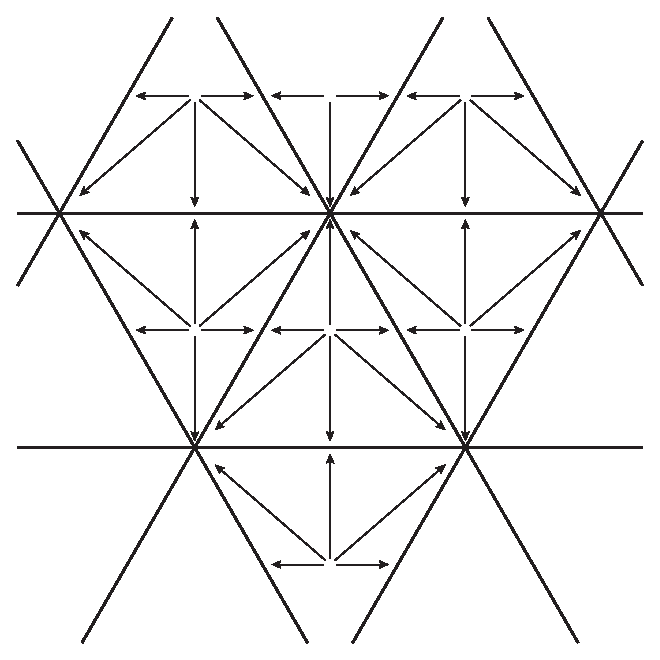
\includegraphics[scale=0.75]{fig/euler-vf-2b}
\caption{Schematic example of $V_T$ in several cells of a triangulation.}
\label{fig:vt-1}
\end{figure}

%In particular, we see that each vertex of the triangulation is a zero of the vector field and this zero acts as a sink and so has index 1. At the centre of each edge is a zero where 
In terms of the figure above, we have that each zero in the centre of a simplex $\delta^i$ is a saddle point which sends flow lines out in an $i$-dimensional hyperplane and receives flow lines from the other higher dimensional $\delta^{i+1}$ simplices. One can show that the index of the zero will be $(-1)^i$ \cite{guillemin2010differential, wrightPoincare}. Summing over all the indices gives,
\begin{align*}
\sum_{x\in V_T^{-1}(0)}\mathrm{Ind}_xV_T&=\sum_{i=1}^m\sum_{i\text{-simplices }S}\mathrm{Ind}_{c_S}V_T\\
&=\sum_i(-1)^is_i\\
&=\chi(M),
\end{align*}
where $c_S$ is the centre point of the simplex $S$.
We hence have for any vector field with a finite number of zeroes,
\[
\sum_{x\in V^{-1}(0)}\mathrm{Ind}_xV=\chi(M).
\]
It immediately follows at this point that if $M$ admits a nowhere vanishing vector field, then $\chi(M)=0$.\\

On the other hand, if $\chi(M)=0$, we know that $V_T$ has the same number of zeroes with index $+1$ as zeroes with index $-1$. We can homotope $V_T$ such that the zeroes are paired together such that every zero of index $+1$ is in a chart domain together with a single zero of index $-1$ and vice versa. 

We may then do the opposite of what the splitting lemma provides and merge the zeroes, effectively canceling each pair out, leaving us with no zeroes at all. In other words, if we take a disk around a pair of such zeroes, we have a degree 0 map on the boundary of that disk and we can extend that map onto the whole disk, leaving us with no zeroes.

This concludes the proof of the theorem.
\end{proof}
Observe that since $\chi(\mathbb{S}^n)=1+(-1)^n$ (see \cite{wrightPoincare}), we have that this also proves the statement that there exists a nowhere vanishing vector field on $\mathbb{S}^n$ if and only if $n$ is odd.

\pagebreak

\subsection{Parallelisations for $\mathbb{S}^1$, $\mathbb{S}^3$ and $\mathbb{S}^7$.}
\begin{proposition}
$\mathbb{S}^1$ is parallelisable.
\end{proposition}
\begin{proof}
By \eqref{eq:novan-vect-1}, we have $V(x,y)=(-y,x)$. If we consider the points of $\mathbb{S}^1$ via the parameterisation $(\cos\theta,\sin\theta)$, then
\[
V(\cos\theta,\sin\theta)=(-\sin\theta,\cos\theta)=\gamma'(\theta),
\] 
where $\gamma(\theta)=(\cos\theta,\sin\theta)$ is a curve on $\mathbb{S}^n$, with $\gamma'(\theta)$ tangent.

Hence, by Proposition \ref{prop:para-condn}, $V(x,y)=(-y,x)$ forms a frame for $\mathbb{S}^1$ and so we have that $\mathbb{S}^1$ is parallelisable.

\begin{figure}[h!]
\centering
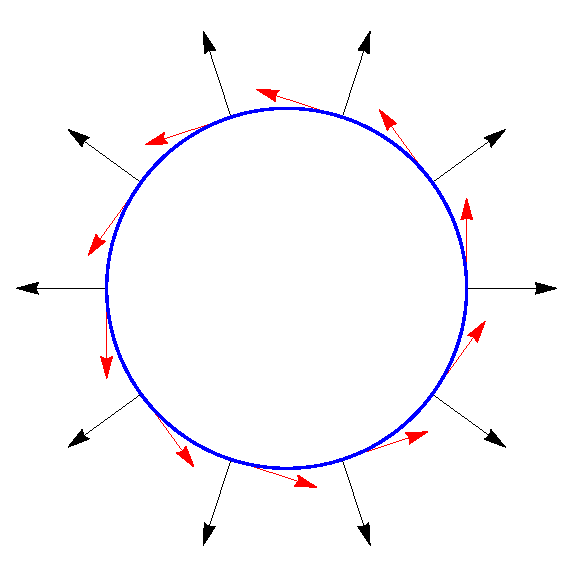
\includegraphics[scale=0.75]{fig/s1-norm-tang}
\caption{$\mathbb{S}^1$ with the vector fields $R$ (black) and $V$ (red).}
\label{fig:s1+norm+tang}
\end{figure}
\end{proof}

\begin{proposition}
$\mathbb{S}^3$ is parallelisable.
\end{proposition}
\begin{proof}
Recall the quaternion number system, $\mathbb{H}$. The quaternions are a four-dimensional, noncommutative number system. To define a product of two elements in $\mathbb{H}$ requires a choice of basis for $\mathbb{R}^4$. Elements of the basis are typically denoted by $1,i,j,k$ and elements of $\mathbb{H}$ are typically written in the form $a+bi+cj+dk$, where $i,j,k$ have the property,
\[
i^2=j^2=k^2=ijk=-1.
\]
Multiplication of $i,j,k$ can be summarised by the following diagram.

\begin{figure}[h!]
\centering
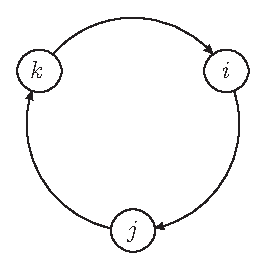
\includegraphics[scale=1]{fig/quat-mult}
\caption{Graphical representation of quaternion multiplication.}
\label{fig:quat-mul}
\end{figure}

For example, $ij=k$, $kj=-i$ and so on.

Since $\mathbb{H}$ may be identified with $\mathbb{R}^4$, we can consider $\mathbb{S}^3$ as the set of unit quaternions,
\[
\mathbb{S}^3=\left\{q=x_1+x_2i+x_3j+x_4k\in\mathbb{H}:\|q\|=1 \right\}.
\]
Considering $\mathbb{S}^3$ as the set of unit quaternions, we have that for any point $q=(x_1,x_2,x_3,x_4)\in\mathbb{S}^3$, the collection $\{iq,jq,kq\}$ forms a frame on $\mathbb{S}^3$. To show this, we compute directly as follows.
\begin{align*}
iq&=i(x_1+x_2i+x_3j+x_4k)\\
&=(ix_1+ix_2i+ix_3j+x_4k)\\
&=(x_1i+x_2i^2+x_3ij+x_4ik)\\
&=(x_1i-x_2+x_3k-x_4j)\\
&=(-x_2,x_1,-x_4,x_3)\\
jq&=j(x_1+x_2i+x_3j+x_4k)\\
&=(jx_1+jx_2i+jx_3j+jx_4k)\\
&=(x_1j+x_2ji+x_3j^2+x_4jk)\\
&=(x_1j-x_2k-x_3+x_4i)\\
&=(-x_3,x_4,x_1,-x_2)\\
kq&=k(x_1+x_2i+x_3j+x_4k)\\
&=(kx_1+kx_2i+kx_3j+kx_4k)\\
&=(x_1k+x_2ki+x_3kj+x_4k^2)\\
&=(x_1k+x_2j-x_3i-x_4)\\
&=(-x_4,-x_3,x_2,x_1)
\end{align*}
To summarise, we have the following three vector fields,
\begin{align*}
V_1&=(-x_2,x_1,-x_4,x_3),\\
V_2&=(-x_3,x_4,x_1,-x_2),\\
V_3&=(-x_4,-x_3,x_2,x_1).
\end{align*}
Note that $V_1$ is precisely the vector field one gets by applying the construction defined by \eqref{eq:novan-vect-1} to the point $q$.\\
%It remains to be shown that these are linearly independent.\\
As with the example of $\mathbb{S}^1$, consider the normal vector field to the sphere given by $N=(x_1,x_2,x_3,x_4)$. Then we have that,
\begin{align*}
\langle N,V_1\rangle&=N\cdot V_1\\
&=(x_1,x_2,x_3,x_4)\cdot (-x_2,x_1,-x_4,x_3)\\
&=-x_2x_1+x_2x_1-x_3x_4+x_4x_3\\
&=0,
\end{align*}
and similarly for $V_2$ and $V_3$. Furthermore, we observe that
\begin{align*}
\langle V_1,V_2\rangle &=V_1\cdot V_3\\
&=(-x_2,x_1,-x_4,x_3)\cdot (-x_3,x_4,x_1,-x_2)\\
&=x_2x_3+x_1x_4-x_4x_1-x_3x_2\\
&=0.
\end{align*}
Similarly, we find that $\langle V_1,V_3\rangle=\langle V_2,V_3\rangle=0$. Hence $V_1$, $V_2$ and $V_3$ are all orthogonal to the normal and hence tangent to the sphere. Furthermore we have that $V_1$, $V_2$ and $V_3$ are all linearly independent. Thus $\{V_1,V_2,V_3\}$ forms a frame on $\mathbb{S}^3$.\\
%To see that $\{V_1,V_2,V_3\}$ is a linearly independent set, consider the following. Since $\{i,j,k\}$ is a linearly independent set, this implies that $\{qi,qj,qk\}$ is a linearly independent set since $L_q:\mathbb{R}^4\to\mathbb{R}^4$ is a linear isomporhism (see the next section for details on this map). \textbf{\textcolor{red}{Bad?}}

As we will see in the next section, this type of construction generalises if we have the structure of a division algebra.
\end{proof}
\begin{proposition}
$\mathbb{S}^7$ is parallelisable.
\end{proposition}
\begin{proof}
Recall the octonions, $\mathbb{O}$. The octonions are an eight-dimensional noncommutative and nonaassociative number system. We can think of the octonions in terms of 8-tuples of real numbers, where each octonion is a real linear combination of basis octonions, $\{1,e_1,\ldots,e_7\}$. Each of the $e_i$ has the property that $e_i^2=-1$.
Multiplication of the basis octonions can be summarised by the following diagram, read in a similar manner to the analogous diagram for quaternions.\\

\begin{figure}[h!]
\centering
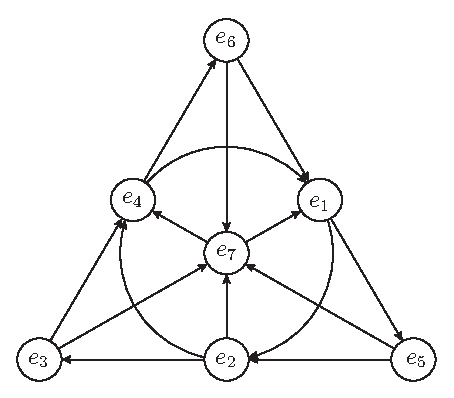
\includegraphics[scale=1]{fig/octo-mult}
\caption{Graphical representation of octonion multiplication.}
\label{fig:octo-mul}
\end{figure}

When we move to the octonions, $\mathbb{O}$, we lose the property of associativity \cite{wirthmuller_2012}. As such, $\mathbb{O}$ cannot be embedded in a matrix algebra. Instead, consider the following. Identify $\mathbb{O}$ with $\mathbb{H}^2$ and define the multiplication by,
\[
(u,v)\cdot(w,z)=(uw-vz^*,uz+vw^*).
\]
Where $q^*$ denotes the conjugate quaternion $q^*=a-bi-cj-dk$.
We have a conjugation $(u,v)\mapsto (u^*,-v)$ which provides the norm, which in turn allows one to write down the inverse of any non-zero octonion with respect to the unit $(1,0)\in\mathbb{O}$.\\

Using the same technique as in the case of $\mathbb{S}^3$, we this time consider $\mathbb{S}^7$ as the set of unit octonions,
\[
\mathbb{S}^7=\left\{q=x_0e_0+x_1e_1\cdots+x_7e_7\in\mathbb{O}:\|q\|=1 \right\},
\]
where $e_i$ are the basis octonions.
%which satisfy multiplication table.
%\begin{table}[]
%\centering
%%\caption{My caption}
%%\label{my-label}
%\begin{tabular}{l|llllllll}
%$e_ie_j$ & $e_1$ & $e_2$ &$e_3$ &$e_4$  &$e_5$  &$e_6$&$e_7$&$e_8$  \\
%\hline
%$e_1$ &$e_1$  &$e_2$  &$e_3$  &$e_4$  &$e_5$  &$e_6$&$e_7$  &$e_8$  \\
%$e_2$ &$e_2$  &$-e_1$  &$e_4$  &$-e_3$  &$e_6$&$-e_5$&$-e_8$&$e_7$  \\
%$e_3$ &$e_3$  &  &$-e_1$  &  &  &  &  &  \\
%$e_4$ &$e_4$  &  &  &$-e_1$  &  &  &  &  \\
%$e_5$ &$e_5$  &  &  &  &$-e_1$  &  &  &  \\
%$e_6$ &$e_6$  &  &  &  &  &$-e_1$  &  &  \\
%$e_7$ &$e_7$  &  &  &  &  &  &$-e_1$  &  \\
%$e_8$ &$e_8$  &  &  &  &  &  &  &$-e_1$ 
%\end{tabular}
%\end{table}

Then for any point $q=(x_0,x_1,\ldots,x_7)\in\mathbb{S}^7$, the set $\{qe_1,qe_2,\ldots,qe_7\}$ forms a frame on $\mathbb{S}^7$.
We forego writing out the entire computation here since it is simply a more tedious variation of the one carried out for $\mathbb{S}^3$.

%After the aforementioned lengthy computation, one yields the following vector fields.
\end{proof}
\begin{remark}
In view of the results presented in the next section, we note here that there was nothing stopping us from constructing the parallelisation of $\mathbb{S}^1$ using the complex numbers, just as the quaternions and octonions were used for $\mathbb{S}^3$ and $\mathbb{S}^7$ - simply take the map $z\mapsto iz$. Given the familiar setting of $\mathbb{R}^2$ and $\mathbb{S}^1$ however, there was little motivation for using this association with $\mathbb{C}$.
\end{remark}

\pagebreak
\subsection{Division Algebras}
In this section, we present some results that closely relate the existence of division algebras with the previously discussed results for sphere parallelisability.
\begin{definition}
A \textit{division algebra} is a ring in which every non-zero element has a multiplicative inverse, but in which multiplication is not necessarily commutative. For more details, see \cite{MR1415833}.
\end{definition}
\begin{theorem}
Suppose $\mathbb{R}^n$ has a division algebra structure, $m:\mathbb{R}^n\times\mathbb{R}^n\to\mathbb{R}^n$. Then $T\mathbb{S}^{n-1}$ is diffeomorphic to $\mathbb{S}^{n-1}\times\mathbb{R}^{n-1}$.
\end{theorem}
\begin{proof}
Suppose $\mathbb{R}^n$ is a division algebra. By definition of a division algebra, we have that there exists an identity element $e\in\mathbb{S}^{n-1}$ such that
\[
m(e,x)=m(x,e)=x,\,\forall x\in\mathbb{R}^n.
\]
For each point $x\in\mathbb{S}^{n-1}$, let us define the map $L_x:\mathbb{S}^{n-1}\to\mathbb{S}^{n-1}$ by,
\[
L_x(y)=\frac{m(x,y)}{\|m(x,y)\|},
\]
given some other point $y\in\mathbb{S}^{n-1}$. Since $\mathbb{R}^{n}$ is a division algebra, for each element $z\in\mathbb{S}^{n-1}$, there exists precisely one other element $y\in\mathbb{S}^{n-1}$ such that $L_x(y)=z$. Hence $L_x$ is a diffeomorphism 
%(\texttt{Is what we have thus far sufficient to conclude this I wonder?}). 
Furthermore, note that $L_x(e)=x$. Hence, we have $d(L_x)_e:T\mathbb{S}^{n-1}_e\to T\mathbb{S}^{n-1}_x$ is a linear isomorphism. Now define the diffeomorphism $f:\mathbb{S}^{n-1}\times T\mathbb{S}^{n-1}_e\to T\mathbb{S}^{n-1}$ by,
\[
f(x,v)=\left(x,d(L_x)_e(v) \right).
\]
We may now conclude that $\mathbb{S}^{n-1}\times T\mathbb{S}^{n-1}_e\cong \mathbb{S}^{n-1}\times\mathbb{R}^{n-1}$ is diffeomorphic to $T\mathbb{S}^{n-1}$.\\
%(\texttt{More detail required?}).

%\texttt{Don't quite buy/need to show}: $\mathbb{S}^{n-1}\times T\mathbb{S}^{n-1}_e\cong\mathbb{S}^{n-1}\times\mathbb{R}^{n-1}$...\\

%In addition, we note that we can always modify the multiplication map $m$ to produce an identity that fits our requirements. Specifically, choose a vector $e\in\mathbb{S}^{n-1}$. After composing the multiplication with an invertible linear map from $\mathbb{R}^n\to\mathbb{R}^n$, taking $m(e,e)$ to $e$, we may assume that $m(e,e)=e$. Let $\alpha$ be the map such that $x\mapsto m(x,e)$ and let $\beta$ be the map such that $x\mapsto m(e,x)$. Now define the new multiplication map $m'$ to be
%\[
%m'(x,y)=m\left(\alpha^{-1}(x),\beta^{-1}(x)\right).
%\]
%Observe that
%\[
%m'(x,e)=m\left(\alpha^{-1}(x),\beta^{-1}(e) \right)=m(\alpha^{-1}(x),e)=x,
%\]
%and
%\[
%m'(e,x)=x.
%\]
%Thus, we have produced a new multiplication map $m':\mathbb{R}^n\to\mathbb{R}^n$ with an identity element $e\in\mathbb{S}^{n-1}$.\\

For each point $x\in\mathbb{S}^{n-1}$, our map $L_x$ gives a linear isomorphism from $\mathbb{R}^n$ to itself. By scaling the output to have length 1, left multiplication by $x$ gives a diffeomorphism from $\mathbb{S}^{n-1}$ to itself which maps the point 1 to $x$. Taking the derivative of this diffeormorphism at the point $1$ gives a linear isomorphism from the tangent space of the sphere at the point $1$ to the tangent space at $x$. Since the point $x$ on the sphere is arbitrary, a choice of basis for the tangent space of the sphere at the point $1$ determines a trivialisation of the whole bundle of the $(n-1)$-sphere. 
\end{proof}
We also have the following alternative characterisation of the same proof which we present here for the sake of contrast.
\begin{theorem}
If $\mathbb{R}^n$ has the structure of a division algebra, then $S^{n-1}$ is parallelisable.
\end{theorem}
\begin{proof}
Choose a basis $\{e_1,\ldots,e_n\}$ of $\mathbb{R}^n$ such that $e_1=1$. Take $x\in\mathbb{S}^{n-1}$ and define
\begin{equation}
v_i(x)=xe_i-\langle x,xe_i\rangle x,\,i\geq 2.
\label{eq:vi-orig}
\end{equation}
Then we have $\langle x,v_i(x)\rangle =0$ and so $(x,v_i(x))\in T\mathbb{S}^{n-1}$, i.e. $v_i$ is a tangent vector field on $\mathbb{S}^{n-1}$. Since,
\[
\{1,e_2,\ldots,e_n\},
\]
is a linearly independent set, so is the set
\[
\{x,xe_2,\ldots,xe_n\},
\]
since we have the structure of a division algebra, meaning that $L_x$ is a linear isomorphism.

%Note that if we consider the $v_i$ as being written in the form $v_{i+1}=c_{i+1}e_i+f_{i+1}$, $v_{i+2}=c_{i+2}e_i+f_{i+2}$ for $i\geq 2$, then if $f_3=\lambda f_2$, for some scalar $\lambda$, then $e_i,e_{i+1}\in\mathrm{span}\{e_i,f_2\}$ and so on. However, since we know that the $e_i$ are linearly independent and by the above, we know that this is not the case. \texttt{TO BE FIXED LATER...}
\begin{proposition}
The vectors $v_i(x)$ form a basis for $T_x\mathbb{S}^{n-1}$.
\end{proposition}
\begin{proof}
Given a point $x\in\mathbb{S}^{n-1}$, it follows that $\{x\}^\bot=T_x\mathbb{S}^{n-1}$, i.e. the set of vectors orthogonal to $x$ on the sphere are precisely those in the tangent space at $x$.
Hence, we have the following characterisation of the vectors $v_i(x)$ in terms of a projection $\pi$ onto the orthogonal complement of $x$.
\[
v_i(x)=\pi_{\{x\}^\bot}(e_i\cdot x)=\pi_{T_x\mathbb{S}^{n-1}}(e_i\cdot x).
\]
First, note that 
\[
\dim\left(\mathrm{span}\{v_i\}_{i=2}^n\right)=n-1=\dim\left(T_x\mathbb{S}^{n-1}\right).
\]
Since the spaces under consideration are finite dimensional, it suffices to show that $\dim \pi(\mathrm{span}\{v_i\}) =n-1$.\\

Let $\{w_j\}_{j=1}^k$ with $k\leq n-1$ be a basis for $\pi(\mathrm{span}\{v_i\})$. Then $v_i=c^j_iw_j$ (where the Einstein summation convention is being used). Rearranging \eqref{eq:vi-orig} for $xe_i$, we hence have,
\begin{align*}
xe_i&=v_i+\langle x,xe_i\rangle x\\
&=c^j_iw_j+\langle x,xe_i\rangle x.
\end{align*}
Note that
\[
c^j_iw_j+\langle x,xe_i\rangle x\in\mathrm{span}\{x,w_j\},
\]
We hence have that
\begin{align*}
\mathrm{span}\{xe_i\}&\subseteq\mathrm{span}\{x,w_j\}\\
\Rightarrow n&=k+1\\
\Rightarrow k&=n-1,
\end{align*}
as was required.
\end{proof}
%We claim that it follows that the vectors $v_2(x),\ldots,v_n(x)$ are linearly independent. To see this, consider the following. Assume for a contradiction that their projections are linearly dependent. Then given $e_1,\ldots,e_{n+1}$, we can write $v_2,\ldots,v_{n+1}$ in the form
%\begin{align*}
%v_2&=c_2e_1+f_2\\
%&\,\,\,\vdots\\
%v_{n+1}&=c_{n+1}e_1+f_{n+1},
%\end{align*}
%where the $c_i$ are constants and the $f_i\in e_1^{\bot}$. Let $V=\mathrm{span}f_i$. Then $e_1,e_2,\ldots,e_{n+1}\in V\bigoplus e_1$. This would imply that the basis vectors $e_i$ are linearly dependent, a contradiction.
Hence, the vectors $v_2(x),\ldots,v_n(x)$ are linearly independent. Consequently, the map $\varphi:\mathbb{S}^{n-1}\times \mathbb{R}^{n-1}\to T\mathbb{S}^{n-1}$ defined by,
\[
\varphi(x,(t_2,\ldots,t_n))=(x,t_2v_2(x)+\cdots+t_nv_n(x)),
\]
is the isomorphism between $T\mathbb{S}^{n-1}$ and $\mathbb{S}^{n-1}\times\mathbb{R}^{n-1}$ that we seek.
\end{proof}
\pagebreak
\section{Generalisations \& Consequences}
At this point we have established the following results.
\begin{enumerate}
\item Even dimensional spheres do not admit a smooth non-vanishing vector field, let alone enough to form a basis for the tangent bundle.
\item Odd dimensional spheres are guaranteed to admit at least one such field.
\item $n$-spheres for $n=1,3,7$ admit 1, 3 and 7 linearly independent, non-vanishing smooth vector fields and hence are parallelisable.
\end{enumerate}
As stated in the historical overview, the now well established, claim is that these are indeed the only parallelisable spheres. It is however, beyond the scope of this project to prove this claim. A summary of the four key works on this particular topic are described chronologically as follows (among the other papers mentioned in the historical overview).
\begin{enumerate}
%\item 1898: Hurwitz's theorem for formulae of sums - \cite{Hurwitz1898}
%\item 1940/1941: Hopf - Dimension of a division algebra is a power of 2 - \cite{MR0004785}
\item January 1958: \cite{MR3075371} - Kervaire uses a theorem due to Bott in order to show that for $s\geq 3$, $\mathbb{S}^{4s-1}$ is not parallelisable. 
\item Februrary 1958: \cite{MR0102805} - Milnor uses the same theorem of Bott's to show that the only division algebras over the reals of dimension $n$ occur only for $n=1,2,4,8$ and that these are the only $n$ for which $\mathbb{S}^{n-1}$ is parallelisable. 
%\item 1958: Bott \& Milnor - Sphere parallelisability - \cite{MR0102804}
\item January 1960: \cite{MR0141119} - Adams uses $K$-theory to establish the equivalence between sphere parallelisability and division algebra existence among two other equivalent concepts. A key point to note is that Adams' work gives insight into parallelisability of $\mathbb{S}^{n-1}$ with differentiable structures other than the standard one.
\item April 1960: \cite{atiyah1961bott} - Atiyah \& Hirzebruch give a refined version of Bott's results to prove that $\mathbb{S}^n$ is not parallelisable for $n\neq 1,3,7$ with the standard differentiable structure. 
\end{enumerate}
The work of Milnor, Kervaire, Atiyah, Hirzebruch and Adams all rely on $K$-theory and in particular, so called Bott Periodicity.
%In order to show rigorously that $n=1,2,4,8$ are indeed the only dimensions in which a division algebra exists or in which $\mathbb{S}^{n-1}$ is parallelisable, we require:\\
%
%In the 19th century, Frobenius and Hurwitz were able to prove that there are only four normed division algebras ($\mathbb{R},\mathbb{C},\mathbb{H},\mathbb{O}$).

%\textit{Rough Timeline of Events:}
%\begin{enumerate}
%\item 1898: Hurwitz's theorem - \cite{Hurwitz1898}
%\item 1940/1941: Hopf - Dimension of a division algebra is a power of 2 - \cite{MR0004785}
%\item 1958: Milnor - Dim is 1, 2, 4 or 8 - \cite{MR0102805}
%\item 1958: Bott \& Milnor - Sphere parallelisability - \cite{MR0102804}
%\item 1958: Kervaire - Nonparallelisability of the sphere $\mathbb{S}^{n-1}$ for $n>8$ - \cite{MR3075371}
%\item 1960: Atiyah \& Hirzebruch - Parallelisability of spheres - \cite{atiyah1961bott}
%\item 1960: Adams - Equivalent conditions - \cite{MR0141119}
%\item 1962: Adams - Vector fields on spheres paper - \cite{MR0139178}
%\end{enumerate}

%\textbf{\textcolor{red}{Probably need to rejig the history section to ensure consistency...}}\\
Topological $K$-Theory is a branch topology that relies primarily on algebaric tools such homology and cohomology in the solution of problems. In particular, it is a form of generalised cohomology theory (a tool which we have not discussed in this report) and is used to study vector bundles on topological spaces. Early work in the field of topological $K$-theory was due to Atiyah and Hirzebruch. 
%In their paper \cite{atiyah1961bott}, Atiyah and Hirzebruch use theorems due to Bott to prove that $\mathbb{S}^n$ is not parallelisable for $n\neq  1,3,7$ with the usual differentiable structures on the sphere.

In \cite{MR0141119}, Adams famously applied topological $K$-theory in order to solve the ``Hopf invariant one problem''. The Hopf invariant is a type of homotopy invariant between spheres. As mentioned in the historical overview, in \cite{MR1512691}, Hopf established a map $\eta:\mathbb{S}^3\to\mathbb{S}^2$ where for any point $x\in\mathbb{S}^2$, the pre-image under $\eta$ is a circle in $\mathbb{S}^3$. Hopf was able to use the linking number (a numerical invariant describing the number of times a curve in space winds around another) of two such circles to prove that $\eta$ is not homotopic to the constant map. From here, the map was generalised to the form $\phi:\mathbb{S}^{2n-1}\to\mathbb{S}^n$, $n>1$. Through the use of (co)homology theory, an integer-valued invariant $h(\phi)$ was developed and a natural question to then pose was ``for which values of $n$ is $h(\phi)=1$?''. It was then in \cite{MR0141119} where Adams was able to answer this question and show that $n=1,2,4,8$ are the only such possible values.

As a result of this, he managed to established strong conditions on, among other things, the existence of division algebras as well as establishing that $S^{n-1}$ with is parallelisable only for $n=2,4,8$.\\
%\subsection{$K$-Theory}

As a final remark, we have the following results closely related to the results discussed in this report.
\begin{itemize}
\item The only fibre bundles in which the total, base and fibre spaces are all spheres are precisely those whose fibre spaces are the parallelisable spheres, i.e.
\begin{itemize}
\item $\mathbb{S}^1\to\mathbb{S}^1$ with fibre $\mathbb{S}^0$,
\item $\mathbb{S}^3\to\mathbb{S}^2$ with fibre $\mathbb{S}^1$,
\item $\mathbb{S}^7\to\mathbb{S}^4$ with fibre $\mathbb{S}^3$,
\item $\mathbb{S}^{15}\to\mathbb{S}^8$ with fibre $\mathbb{S}^7$,
\end{itemize} 
are the only such types of fibre bundles. This is a consequence of Adams.
\item All Lie groups (i.e. smooth manifolds also endowed with a group structure) are parallelisable, \cite{MR2954043}. It is interesting to note that while $\mathbb{S}^1$ and $\mathbb{S}^3$ have Lie group structures, $\mathbb{S}^7$ does not.
\item All parallelisable manifolds are orientable. A proof of this can be found in \cite{MR2954043}.
\end{itemize} 

%\textcolor{red}{Hopf maps, hopf invariant, Adams...}
%
%If one is familiar with the concept of a \textit{Lie group} (i.e. a manifold also endowed with a group structure), \textcolor{red}{something something something all Lie groups are parallelisable...} $\mathbb{S}^3$ has a Lie group structure but $\mathbb{S}^7$ does not.
%
%Furthermore, it can be shown that all parallelisable manifolds are orientable. For a proof of this, refer to \cite{MR2954043}.
%\subsection{Consequences}
%%\textcolor{red}{Existence of parallel transport on manifolds due to parallelisability?}\\
%
%\textcolor{red}{All parallelisable manifolds are orientable.}\\
%
%\textcolor{red}{Every Lie Group is parallelisable.}\\
%
%\textcolor{red}{Hopf maps?}
\pagebreak

\section{Conclusion}
In this report, we have discussed the parallelisability of spheres. We first showed that no even dimensional sphere is capable of admitting such a parallelisation and in doing so, proved the famous Hairy Ball Theorem. We showed that odd dimensional spheres, $\mathbb{S}^1$, $\mathbb{S}^3$ and $\mathbb{S}^7$ do admit parallelisations. As stated in the previous section, we claimed that these are indeed the only parallelisable spheres but in order to actually show that $\mathbb{S}^n$ for $n=1,3,7$ are indeed the only cases, we must refer to the work of Milnor and Bott, or Hirzebruch and Kervaire or Adams. We have also briefly discussed the relationship between these parallelisable spheres and the existence to division algebras and related results.

\clearpage

%\addcontentsline{toc}{section}{References}
\bibliographystyle{alpha}
\bibliography{ref1}
\end{document}
